\chapter{交流电}
我们已经学过了直流电,除了直流电,还有大小和方向
都随时间作周期性变化的电流,叫做\textbf{交流电},交流电比起
直流电来有许多优点,交流电可以利用变压器升高或者降低
电压,交流电可以驱动结构简单、运行可靠的感应电动机,因
此在工农业生产和日常生活中普遍使用交流电.这一章我们
就来学习交流电.

交流电和直流电都是电荷定向移动形成的,它们存在着
共同点.学习交流电,应该注意这种共同点.但是交流电不
同于直流电,有它自己的特点.正是这些特点使交流电具有
上述优点.学习交流电,更要注意它的特点.

\section{交流电的产生}


法拉第发现的电磁感应现象的一个重大应用是制成发电
机.交流电就是从交流发电机发出的.

我们在初中学过,照图3.1那样,使矩形线圈$ABCD$在匀
强磁场中匀速转动,电流表的指针就随着线圈的转动而左右
摆动,表明电路里产生了交流电.

\begin{figure}[htp]\centering
    \includegraphics[scale=1.1]{fig/3-1.pdf}
    \caption{交流电的产生}
    \end{figure}

线圈在磁场中转动时,它的$AB$边和$CD$边切割磁力线,在
线圈中产生感生电动势,在电路中就产生感生电流.当线圈
平面转到图3.1乙所示的位置时,$AB$边向下运动,$CD$边向上
运动,感生电动势和感生电流的方向如图中所示.线圈转过
半周,当线圈平面转到图3.1丁所示的位置时,$AB$边变成向
上运动,$CD$边变成向下运动,感生电动势和感生电流的方向
都发生了改变.当线圈平面转到跟磁力线垂直的平面时(图3.1甲和丙),在
这一时刻,$AB$边和$CD$边的线速度方向跟磁力线平行,都不切
割磁力线,因而没有感生电动势和感生电流.跟磁力线垂直
的这个平面叫做\textbf{中性面},线圈平面每经过中性面一次,感生电
动势和感生电流的方向就改变一次,因此,线圈转动一周,感
生电动势和感生电流的方向改变两次.

图3.1其实就是一个交流发电机的模型.实际的发电机,
结构比较复杂,但发电机的基本组成部分仍是线圈(通常叫电
枢)和磁极.电枢转动、磁极不动的发电机,叫做旋转电枢式
发电机,磁极转动,而电枢不动,线圈依然切割磁力线,电枢
同样会产生感生电动势,这种发电机叫旋转磁极式发电机.不
论哪种发电机,转动的部分都叫转子,不动的部分都叫定子.

旋转电枢式发电机,转子产生的电流必须经过裸露着的
滑环和电刷引到外电路,如果电压很高,就容易发生火花放
电,有可能烧毁电机.同时,电枢可能占有的空间也受到限
制,线圈匝数不能很多,产生的感生电动势不能很高.这种发
电机提供的电压一般不超过500伏.旋转磁极式发电机克服
了上述缺点,能够提供几千到几万伏的电压,输出功率可达几
十万千瓦,所以大型发电机都是旋转磁极式的.

发电机的转子是由蒸汽轮机、水轮机或其他动力机带动
的,动力机将机械能传递给发电机,发电机把机械能转化为
电能输送给外电路.

\section{交流电的变化规律}

\begin{figure}[htp]\centering
    \begin{tikzpicture}[>=latex, scale=1.5]
    
    \foreach \x in {.25,.75,-.25,-.75}
    {
        \draw[->] (-2,\x)--(2,\x);
    }

\draw[->] (150:1.5)--+(-120:.8) node [below]{$v$};
\draw[->] (-30:1.5)--+(60:.8) node [above]{$v$};

\draw (.75*1.732+.25, -0.75)arc (0:60:.25)node [right]{$\omega t$};

 \node at (120:2.2) {$\omega t$};

    \draw [dashed](0,-1.5)--(0,2.5)node [right]{中性面};
    \draw [dashed] (0,0)--(-30:2.2); \draw [dashed] (0,0)--(150:2.2);

    \draw[rotate=-30] (-1.5,-.07)node[below]{$d$} rectangle (1.5,.07)node[above]{$a$};
    \draw[rotate=-30, fill=white] (-1.5,0) circle (2.5pt) node{\tiny$\cdot$};
    \draw[rotate=-30, fill=white] (1.5,0) circle (2.5pt) node{\tiny$\times$};

\node at (2.5,0){$B$};


\draw [<->] (0,2) arc (90:150:2) ;


    \end{tikzpicture}
    \caption{}
    \end{figure}

现在我们来研究交流电的变化规律.图3.2中标$a$的小
圆圈表示线圈$ab$边的横截面,标$d$的小圆圈表示线圈$cd$边
的横截面.假定线圈平面从中性面开始转动,角速度是$\omega$(弧
度/秒),经过时间$t$,线圈转过的角度是$\omega t$,$ab$边的线速度$v$
的方向跟磁力线方向间的夹角也等于$\omega t$.设$ab$边的长度是$\ell$,
磁感应强度是$B$,$ab$边中的感
生电动势就是
\[e_{ab}=B\ell v\sin \omega t\]
$cd$边中的感生电动势跟$ab$边
中的大小相同,而且两边又是
串联的,所以这一瞬间整个线
圈中的感生电动势$e$可用下式
表示:
\[e=2B\ell v\sin \omega t\]

当线圈平面转到跟磁力线平行的位置时,$ab$边和$cd$边的
线速度方向都跟磁力线垂直,两边都垂直切割磁力线.这时,
\[\omega t=\frac{\pi}{2},\qquad \sin \omega t=1 \]
感生电动势最大,用$\mathcal{E}_m$来表示,即
$\mathcal{E}_m=2B\ell v$,把它代入上式就得到
\begin{equation}
    e=\mathcal{E}_m \sin\omega t
\end{equation}
式中的$e$随着时间而变化,不同时刻有不同的数值,叫做电动
势的\textbf{瞬时值},$\mathcal{E}_m$叫做电动势的\textbf{最大值}.上式表明,电动势是
按照正弦规律变化的.

这时电路中电流强度也是按照正弦规律变化的,设整个
闭合电路的电阻为$R$,电流的瞬时值
\[i=\frac{e}{R}=\frac{\mathcal{E}_m}{R} \sin\omega t \]
其中$\mathcal{E}_m/R$是电流的最大值,用$I_m$表示,所以
\begin{equation}
    i=I_m \sin\omega t
\end{equation}

外电路中一段导线上的电压同样是按照正弦规律变化
的,设这段导线的电阻为$R'$,电压的瞬时值
\[u=iR'=I_mR'\sin\omega t \]
其中$I_mR'$是电压的最大值,用$U_m$表示,所以
\begin{equation}
    u=U_m \sin\omega t
\end{equation}

\begin{figure}[htp]\centering
    \begin{tikzpicture}[>=latex, scale=1.5]
    
    \foreach \x in {.25,.75,-.25,-.75}
    {
        \draw[->] (-2,\x)--(2,\x);
    }
    \draw [dashed](0,-1.5)--(0,2.5)node [right]{中性面};
    \draw (0,0)--(-30:1.5); \draw (0,0)--(150:2.2);
\draw[dashed] (120:1.5)--(-60:1.5);
    \draw[rotate=-60, dashed] (-1.5,-.07) rectangle (1.5,.07);
    \draw[rotate=-30] (-1.5,-.07)node[below]{$d$} rectangle (1.5,.07)node[above]{$a$};
    \draw[rotate=-30, fill=white] (-1.5,0) circle (2.5pt) node{\tiny$\cdot$};
    \draw[rotate=-30, fill=white] (1.5,0) circle (2.5pt) node{\tiny$\times$};
    \draw[rotate=-60, fill=white] (-1.5,0) circle (2.5pt) node{\tiny$\cdot$};
    \draw[rotate=-60, fill=white] (1.5,0) circle (2.5pt) node{\tiny$\times$};
\node at (2.5,0){$B$};

\draw [<->] (0,1.3) arc (90:117:1.3) node [right]{$\phi_0$};
\draw [<->] (0,2) arc (90:150:2) ;
\node at (120:2.2){$\omega t+ \phi_0$};

    \end{tikzpicture}
    \caption{}
    \end{figure}

上述各式都是从线圈平面
跟中性面重合的时刻开始计时
的,如果不是这样,而是如图
3.3所示从线圈平面跟中性面
有一夹角$\phi_0$时开始计时,那么,
经过时间$t$,线圈平面跟中性
面间的角度是$\omega t+\phi_0$,感生电动势的公式就变成
\begin{equation}
    e=\mathcal{E}_m \sin (\omega t+\phi_0)
\end{equation}
电流和电压的公式分别变成
\begin{align}
    i&=I_m\sin (\omega t+\phi_0) \\
    u&=U_m\sin (\omega t+\phi_0)
\end{align}

公式(3.1)、(3.2)、(3.3)或者(3.4)、(3.5)、(3.6),表示交流电是按照正弦规律变化的,这种按照正弦规律变化的交流电叫做\textbf{正弦交流电}.正弦交流电是一种最简单而又最基本的交流电,正如同简谐振动是一种最简单而又最基本的振动一样.
	
	
交流电的变化规律也可以用图象直观地表示出来,图3.4是交变电动势$e=\mathcal{E}_m \sin \omega t$的图象,图象上方画出了对应于交变电动势等于零或正、负最大值时的线圈位置,图3.5是交变电流$i=I_m\sin(\omega t+\phi_0)$或交变电压 $u=U_m\sin(\omega t+\phi_0)$的图象,其中$\phi_0=\pi/6$.
\begin{figure}[htp]\centering
\includegraphics[scale=.75]{fig/3-4.png}
\caption{$e=\mathcal{E}_m \sin \omega t$的图象}
\end{figure}
\begin{figure}[htp]\centering
\begin{tikzpicture}[>=latex, xscale=.7]

\draw[->] (-1,0)--(11,0)node [right]{$\omega t$};
\draw[->] (3.1416/6, -1.5)--(3.1416/6, 2.5)node [above]{$i,u$};
\foreach \x in {3.1416*7/6, 3.1416*13/6, 3.1416*19/6}
{
   \draw (\x, -.1)--(\x, .1);
}
\draw [ultra thick] plot[domain=0:3*3.1416, samples=1000] function{1.5*sin(x)} ;
\draw[dashed](0,-1)--(0,0);

\node at (3.1416/12, -.5){$\phi_0$};
\node at (3.1416/12, -2){$\phi_0=\pi/6=30^{\circ}$};
\draw[->] (-.5,-.5)--(0,-.5);
\draw[->] (3.1416/6+.5,-.5)--(3.1416/6,-.5);
\node at  (3.1416/6+.25,.25) {$O$};
\end{tikzpicture}
\caption{$i=I_m\sin(\omega t+\phi_0)$或$u=U_m\sin(\omega t+\phi_0)$的图象}
\end{figure}



\subsection*{练习一}
\begin{enumerate}
    \item 有人说线圈平面转到中性面的瞬间,穿过线圈的磁通量最大,因而线圈中的感生电动势最大;线圈平面跟中性面垂直的瞬间,穿过线圈的磁通量为零,因而线圈中的感生电动势为零,这种说法对不对?为什么?
    \item 在图3.1所示的实验中,在不改变$B$、$\ell$和$v$的数值的情况下,你有什么办法来提高电动势的最大值?并说明所依据的原理.
    \item 在图3.1所示的实验中,设$AB$边的长度为20厘米,线圈的宽$AD$为10厘米,磁感应强度$B$为0.01特,线圈的转数为50转/秒,求电动势的最大值,如果从线圈平面转过中性面30$^\circ$角的瞬时开始计时,经过0.01秒时电动势的瞬时值是多大?
    \item 画出$u=30\sin(\omega t+\pi/2)$伏的电压图象和$i=2\sin(\omega t-\pi/4)$安的电流图象,以$\omega t$为横轴.
    \item 图3.1是一个发电机模型,只能供课堂演示之用,如果你有兴趣,可约请几位同学,共同研究一下怎样在此模型的	
	基础上加以改进,设计一个小发电机,如果感到知识不足,可自学或查阅有关电工学的书籍.
\end{enumerate}


\section{表征交流电的物理量}

稳恒电流不随时间而变化,要描述电路中的电流或电压,只要指出电流强度或电压的数值就够了,交流电则不然,交流电的电流或电压,大小和方向都随时间作周期性的变化,要描述它们,需要的物理量就要多些,下面讨论表征正弦交流电的物理量.

\subsection{最大值和有效值}

交流电的最大值$(I_m,U_m)$是交流电在一周期内所能达到的最大数值,可以用来表示交流电的电流强弱或电压高低,在实际中有重要意义,例如把电容器接在交流电路中,就需要知道交变电压的最大值,电容器所能承受的电压要高于交变电压的最大值,否则电容器可能被击穿.但是,在研究交流电的功率时,最大值用起来却不够方便,它不适于用来表示交流电产生的效果,在电工技术中通常用有效值来表示交流电的大小.

交流电的有效值是根据电流热效应来规定的,让交流电和直流电通过相同阻值的电阻,如果它们在相同时间内产生的热量相等,就把这一直流电的数值叫数这一交流电的\textbf{有效值}.例如某一交变电流通过一段电阻丝,在一段时间内产生的热量为$Q$,如果改用3安的直流电通过这段电阻丝,在相同的时间内产生的热量也为$Q$,那么,这一交变电流的有效值就
是3安,交流电压的有效值可以用同样的方法来确定,通常用$I$和$U$分别表示交变电流和电压的有效值.这样,知道了交流电的有效值,很容易求出交流电通过电阻时产生的热量.设电流的有效值为$I$,电阻为$R$,在时间$t$内产生的热量$Q=I^2Rt$.这跟直流电路中焦耳定律的形式完全相同,所不同的是在交流电中电流要用有效值.

计算表明,正弦交流电的有效值与最大值之间有如下的关系:
\[\begin{split}
   I&=\frac{I_m}{\sqrt{2}}=0.707I_m\\
   U&=\frac{U_m}{\sqrt{2}}=0.707U_m 
\end{split}\]

我们通常说照明电路的电压是220伏,便是指有效值,各种使用交流电的电气设备上所标的额定电压和额定电流的数值,一般交流电流表和交流电压表测量的数值,也都是有效值,以后提到交流电的数值,凡没有特别说明的,都是指有效值.

\subsection{周期和频率}

跟别的周期性过程一样,交流电也要用周期或频率来表示变化的快慢,在图3.1所示的实验里,线圈匀速转动一周,电动势、电流都按正弦规律变化一周,我们把交流电完成一次周期性变化所需的时间,叫做交流电的\textbf{周期},通常用$T$表示,单位是秒,交流电在1秒钟内完成周期性变化的次数,叫做交流电的\textbf{频率},通常用$f$表示,单位是赫兹.

根据定义,周期和频率的关系是
\[T=\frac{1}{f},\qquad f=\frac{1}{T}\]
	
我国工农业生产和生活用的交流电,周期是0.02秒,频
率是50赫,电流方向每秒改变100次.

\subsection{相和相差}

从交流电瞬时值的表达式可以看出,交流电瞬时值何时为零,何时最大,不是简单地由时间$t$来确定,而是由$\omega t+\phi_0$来确定的.这个相当于角度的量$\omega t+\phi_0$对于确定交流电的大小和方向起着重要作用,叫做交流电的\textbf{相}.相,又叫相位、位相或周相,$\phi_0$是$t=0$时的相,叫做\textbf{初相}.在交流电中,相这个物理量可以用来比较交流电的变化步调.

两个交流电的相位之差叫做它们的\textbf{相差},用$\Delta \phi$来表示.如果交流电的频率相同,相差就等于初相之差,即
\[\Delta \phi=(\omega t+\phi_1)-(\omega t+\phi_2)=\phi_1-\phi_2 \]
这时相差是恒定的,不随时间而改变.

两个频率相同的交流电,如果它们的相位相同,即相差为零,这两个交流电叫做\textbf{同相}的,这两个交流电的变化步调一致,同时到达零和正负最大值(图3.6).	
\begin{figure}[htp]\centering
    \begin{tikzpicture}[>=latex, xscale=.6]
        \draw [->](-2,0)--(6,0)node[right]{$\omega t$};
        \draw [->](0,-1.5)--(0,1.5)node[right]{$i$};
        \draw [ultra thick] plot[domain=0:5.3, samples=1000] function{sin(x+1)} ;
        \draw [ultra thick, dashed] plot[domain=-1:0, samples=100] function{sin(x+1)};
        \node at (2,1) [below]{$i_1$};
        \draw [very thick] plot[domain=0:5.3, samples=1000] function{.7*sin(x+1)} ;
        \draw [very thick, dashed] plot[domain=-1:0, samples=100] function{.7*sin(x+1)};
        \node at (1,.5)[below]{$i_2$};
        \draw [dashed] (-1,0)--(-1,-1.5);
        \draw [<->] (0,-1)--node[above]{$\phi_0$}(-1, -1);

\end{tikzpicture}
\caption{图中的$i_1=I_m\sin(\omega t+\phi_0)$,$i_2=I'_m\sin(\omega t+\phi_0)$}
\end{figure}

两个频率相同的交流电,如果相差为180$^\circ$,即$\Delta\phi=\pi$,这两个交流电叫做\textbf{反相}的.这两个交流电的变化步调恰好相反(图3.7):一个到达正的最大值,另一个恰好到达负的最大值;一个减小到零,另一个恰好增大到零.
\begin{figure}[htp]\centering
    \begin{tikzpicture}[>=latex, xscale=.8]
        \draw [->](-2,0)--(6,0)node[right]{$\omega t$};
        \draw [->](0,-1.5)--(0,1.5)node[right]{$i$};
        \draw [ultra thick] plot[domain=0:5.3, samples=1000] function{sin(x+1)} ;
        \draw [ultra thick, dashed] plot[domain=-1:0, samples=100] function{sin(x+1)};
        \node at (2,1) [below]{$i_1$};
        \draw [very thick] plot[domain=0:5.3, samples=1000] function{-.7*sin(x+1)} ;
        \draw [very thick, dashed] plot[domain=-1:0, samples=100] function{-.7*sin(x+1)};
        \node at (1,-.55)[below]{$i_2$};
        \draw [dashed] (-1,0)--(-1,-1.5);
        \draw [<->] (0,-1)--node[above]{$\phi_0$}(-1, -1);

\end{tikzpicture}
\caption{图中的$i_1=I_m\sin(\omega t+\phi_0)$,$i_2=I'_m\sin(\omega t+\phi_0+\pi)$}
\end{figure}

图3.8表示两个频率相同的交流电,但初相不同,且$\phi_1>\phi_2$.从图中可以看出,这两个交流电的变化步调不一致,$i_1$比$i_2$先到达正的最大值,零或负的最大值.这时我们说$i_1$比$i_2$超前$\Delta\phi$角,或者$i_2$比$i_1$落后$\Delta\phi$角.
\begin{figure}[htp]\centering
    \begin{tikzpicture}[>=latex, xscale=1]
        \draw [->](-2,0)--(7,0)node[right]{$\omega t$};
        \draw [->](0,-1.5)--(0,1.5)node[right]{$i$};
        \draw [ultra thick] plot[domain=0:5.3, samples=1000] function{sin(x+1)} ;
        \draw [ultra thick, dashed] plot[domain=-1:0, samples=100] function{sin(x+1)};
        \node at (1,1) [above]{$i_1$};
        \draw [very thick] plot[domain=0:5.3+.5, samples=1000] function{.7*sin(x+.5)}node [above]{$i_2$} ;
        \draw [very thick, dashed] plot[domain=-.5:0, samples=100] function{.7*sin(x+.5)};
        \draw [dashed] (-1,0)--(-1,-1.5);\draw [dashed] (-.5,0)--(-.5,-1);
        \draw [<->] (0,-1.2)--node[below]{$\phi_1$}(-1, -1.2);
        \draw [<->] (0,-.65)--node[above]{$\phi_2$}(-.5,-.65);
        \draw [<->] (-1,-.75)--node[above]{$\Delta \phi$}(-.5,-.75);


\end{tikzpicture}
\caption{图中的$i_1=I_m\sin(\omega t+\phi_1)$,$i_2=I'_m\sin(\omega t+\phi_2)$}
\end{figure}

最大值(或有效值)、频率(或周期)、初相是表征正弦交流电的三个重要物理量,知道了这三个量,就可以写出交流电瞬时值的表达式,从而知道正弦交流电的变化规律.

\subsection*{练习二}
\begin{enumerate}
    \item 有一个电容器,能耐压250伏,是否能接在220伏的交流电路上?为什么?
    \item 线圈转动的角速度$\omega$也叫角频率(或圆频率),试就图3.1导出角频率$\omega$跟周期$T$或频率$f$的关系式.
    \item 已知:$u_1=220\sqrt{2}\sin(100\pi t+\pi /6)$伏,$u_2=380\sqrt{2}\sin(100\pi t+\pi /3)$伏,求这两个交流电压的最大值、有效值、周期、频率、角频率和初相.这两个电压哪个超前?相差是多大?
    \item 有一正弦交流电,频率是50赫,有效值是5安,初相
    是$-\pi/2$.写出瞬时值的表达式,并画出图象.
    \item 图3.9是某一正弦交流电的图象.根据图象求出最大值、有效值、周期、角频率和初相,并写出瞬时值的表达式.
    \begin{figure}[htp]\centering
        \begin{tikzpicture}[>=latex, xscale=.6]
    \draw [->](-.5,0)--(8.5,0)node[right]{$t$(s)};
    \draw [->](0,-1.5)--(0,2.5)node[right]{$i$(A)};
    \draw [ultra thick] plot[domain=0:3.14*2.5, samples=1000] function{cos(x)};
    \draw [dashed](0,1)--(2*3.1416,1);
    \draw [dashed](0,-1)--(3.1416,-1);
    \node at (0,1) [left]{$+10$};
    \node at (0,-1) [left]{$-10$};
    \foreach \x in {0.05,0.1,0.15,0.2,0.25}
    {
        \node at (\x*31.416, 0)[below]{$\x$};
        \draw(\x*31.416, 0)--(\x*31.416, .1);
    }
    \node at (-.25,-.25){$0$};
    
    \end{tikzpicture}
    \caption{}
    \end{figure}
    \item 图3.10是两个正弦交流电的图象,哪个超前,哪个落后?超前或落后的角度是多大?其中$\phi_1$和$\phi_2$的绝对值都是60$^\circ$.
    \begin{figure}[htp]\centering
        \begin{tikzpicture}[>=latex, xscale=.6]
    \draw [->](-2,0)--(10,0)node[right]{$\omega t$};
    \draw [->](0,-1.5)--(0,1.5)node[right]{$i$};
    \draw [ultra thick] plot[domain=0:9, samples=1000] function{-cos(x+.7)*.7} node [above]{$i_2$};
    \draw [ultra thick] plot[domain=0:8.5, samples=1000] function{sin(x+1)} node [below]{$i_1$};
    \draw [ultra thick, dashed] plot[domain=-1:0, samples=100] function{-cos(x+.7)*.7};
    \draw [ultra thick, dashed] plot[domain=-1:0, samples=100] function{sin(x+1)};
    \node at (-.25,-.25){$O$};
    \draw [dashed] (-1,0)--(-1,-1.5);
    \draw [dashed] (3.1416/2-.7,0)--(3.1416/2-.7,-1.5);
    \draw [<->] (0,-1)--node[below]{$\phi_1$}(-1, -1);
    \draw [<->] (0,-1)--node[below]{$\phi_2$}(3.1416/2-.7,-1);
    
    \end{tikzpicture}
    \caption{}
    \end{figure}
    
\end{enumerate}

\section{纯电阻电路}
交流电路中如果只有电阻,这种电路就叫做\textbf{纯电阻电路}.白炽电灯、电炉、电烙铁等的电路,就是纯电阻电路.

纯电阻电路中电流跟电压的关系,前面已经用过,这里我们再归结一下,把问题明确起来.在纯电阻电路中,在任一时刻电流跟电压的关系都服从欧姆定律,设电阻为$R$,加在它上面的交变电压是$u=U_m\sin \omega t$,通过这个电阻的电流的瞬时值为
\[i=\frac{u}{R}=\frac{U_m}{R}\sin\omega t=I_m\sin\omega t\]
式中$I_m=U_m/R$,如果都换用有效值,就得到
\begin{equation}
    I=\frac{U}{R}
\end{equation}
这就是纯电阻电路中欧姆定律的表达式.这个表达式跟直流电路中欧姆定律的形式完全相同,所不同的是在交流电路中
电压和电流要用有效值.在图3.11所示的电路中通以交流电,用伏特表和安培表量出电压和电流,可以证实上述表达式是正确的.
\begin{figure}[htp]\centering
    \begin{circuitikz}[european]
        \draw (0,0)--(3,0);
        \draw (3,0) to [R=$R$] (3,3);
        \draw (0,3)--(1,3) to [rmeter, t=A] (3,3);
        \draw (1,0) to [rmeter, t=V, *-*] (1,3);
        \draw (0,0)--(0,1.3); \draw (0,1.7)--(0,3);
        \draw (0,1.3) [fill=white]circle (1.5pt);
        \draw (0,1.7) [fill=white]circle (1.5pt);
        \node at (0,1.5){$\sim$};
    \end{circuitikz}\qquad\qquad 
    \begin{tikzpicture}[>=latex, xscale=.7]
        \draw [->](-.5,0)--(8,0)node[right]{$\omega t$};
        \draw [->](0,-1.5)--(0,1.5)node[right]{$i, u$};
        \draw [ultra thick] plot[domain=0:3.1416*2, samples=1000] function{sin(x)};
        \draw [very thick] plot[domain=0:3.1416*2, samples=1000] function{.6*sin(x)};
\node at (1.7,1.2){$u$};
\node at (4.9,-.4){$i$};
\end{tikzpicture}
\caption{}
\end{figure}

在纯电阻电路中,电流和电压是同相的,即电阻对电流和电压的相位关系没有影响.在图3.12所示的实验中,如果用手摇发电机或低频交流电源给电路通以低频交流电,可以看到电流表和电压表的指针的摆动步调一致,表示电流和电压是同相的.
\begin{figure}[htp]\centering
\includegraphics[scale=.75]{fig/3-12.png}
\caption{}
\end{figure}

纯电阻电路中交流电的功率也容易计算出来,在纯电阻
电路中,电能全部转化成内能,电功等于电热,因此,求出单位时间内的电热,就得到交流电的功率.现在用$P$表示交流电的功率,则$P=I^2R$.把$U=IR$代入上式得到
\begin{equation}
    P=UI
\end{equation}

我们看到,在纯电阻电路中,功率的表达式跟直流电路中的形式完全相同,所不同的是在交流电路中电流和电压要用有效值,上述表达式也可以用实验证实.在图3.13所示的电路中,标有$W$的仪表叫瓦特表,是用来测量功率的,接通电路后,把瓦特表的读数跟安培表和伏特表的读数加以比较,就可以知道$P=UI$.
\begin{figure}[htp]\centering
    \begin{circuitikz}[european]
        \draw (0,0)--(5,0);
        \draw (5,0) to [R=$R$] (5,3);
        \draw (5,3)--(4,3) to [rmeter, t=A] (1,3);
        \draw (3.5,0) to [rmeter, t=V, *-*] (3.5,3);
        \draw (0,0)--(0,1.3); \draw (0,1.7)--(0,3);
        \draw (0,1.3) [fill=white]circle (1.5pt);
        \draw (0,1.7) [fill=white]circle (1.5pt);
        \draw (.2,3) [fill=black]circle (1.5pt);
        \node at (0,1.5){$\sim$};
        \draw(1,3) to  (1,0); \draw(1,3)--(1,3.7)--(.2,3.7)--(.2,3);
        \draw (2,3) to [rmeter, t=W, fill=white] (0,3);

    \end{circuitikz}
\caption{}
\end{figure}

在纯电阻电路中,既然欧姆定律的公式和功率的公式跟直流电路中相同,纯电阻电路中的计算就跟直流电路中的计算相同.以前在直流电那一章里所作的计算,有不少本来就是纯电阻电路中的问题,例如关于白炽电灯的计算就是.

需要注意的是:公式(3.6)和(3.7)只适用于纯电阻电路,不适
用于其他交流电路,在其他交流电路中有类似的公式,下面就会学到.	
	
\subsection*{练习三}
\begin{enumerate}
    \item 把“220V,40W”的灯泡接到照明电路中,通过灯泡的电流的最大值是多大?
    \item 在电阻$R$的两端加交变电压$u=220\sqrt{2}\sin(\omega t+\phi)$伏,$R=110$欧,写出电流瞬时值的表达式.
    \item 在电阻为500欧的电阻丝中通以交流电,每秒钟产生5焦的热.求电流和电压的有效值和最大值,交流电的功率是多大?
    \item 把一个电热器接到10伏的直流电路中,每秒钟产生的热量为$Q$.现在把它改接到交流电路中,每秒钟产生的热量为$Q/2$,求交流电压的最大值.
\end{enumerate}

\section{纯电感电路}
在直流电路中,影响电流跟电压关系的只有电阻.在交流电路中,情况要复杂一些,影响电流跟电压关系的,除了电阻,还有电感和电容.	
	
\subsection{电感对交流电的阻碍作用} 
\begin{figure}[htp]\centering
\begin{circuitikz}[>=latex]
\draw (0,1)--(0,.5)--(5,.5)--(5,2) ;
\draw  (3.5,2) to [lamp] (2,2)--(2,1)--(1,1);
\draw [american](3.5,2) to [cute choke, l=$L$] (5,2);

\draw (0,.2)--(0,-1); \draw (1,.2)--(1,-1);
\draw (0,1.8)--(0,3) node[above]{$-$}; \draw (1,1.8)--(1,3)node[above]{$+$};

\node at (-.5,1){$K$};
\draw [ultra thick](0,1)--(-.4,1.8);
\draw [ultra thick](1,1)--(1-.4,1.8);
\draw (-.2, 1.5)-- (-.2+1, 1.5);
\draw [very thick] (-.25, 1.5)-- (-.25+1, 1.5);
\draw [very thick] (-.3, 1.6)-- (-.3+1, 1.6);

\foreach \x in {0,1}
\foreach \y in {.2,-1,1,1.8,3}
{
\draw [fill=white](\x,\y) circle (1.5pt);
}
\node at (.5, -1){$\sim$};


\end{circuitikz}
\caption{}
\end{figure}

如图3.14所示,把电感线圈$L$和白炽灯泡串接在电路里.利用双刀双掷开关$K$可以分别把这个电路接到直流电源或交流电源上,实验中取直流电压和交变电压的有效值相等.实验表明,接通直流电源时,灯泡亮些;接通交流电源时,灯泡变暗,这表明电感对交流电有阻碍作用.

为什么电感对交流电有阻碍作用呢?交流电通过电感线圈时,电流时刻在改变,电感线圈中必然产生自感电动势,阻
碍电流的变化,这样就形成了对电流的阻碍作用.

\subsection{感抗}

在电工技术中,变压器、电磁铁等的线圈,一般是用铜线绕的,铜的电阻率很小,在很多情况下,线圈的电阻比较小,可以略去不计,而认为线圈只有电感.有电感的电路叫\textbf{纯电感电路}.
\begin{figure}[htp]\centering
    \begin{circuitikz}[european]
        \draw (0,0)--(3,0);
        \draw (3,3) to [cute choke] (3,0);
        \draw (0,3)--(1,3) to [rmeter, t=A] (3,3);
        \node at (2.7,1.5){$L$};
        \draw (1,0) to [rmeter, t=V, *-*] (1,3);
        \draw (0,0)--(0,1.3); \draw (0,1.7)--(0,3);
        \draw (0,1.3) [fill=white]circle (1.5pt);
        \draw (0,1.7) [fill=white]circle (1.5pt);
        \node at (0,1.5){$\sim$};
    \end{circuitikz}
\caption{}
\end{figure}
	
现在我们用图3.15所示的电路来研究纯电感电路中电流跟电压的关系.电路中的$L$是电阻可以路去不计的电感线圈.改变交流电源的电压,通过$L$的电流就随着改变.记下几组相应的电流和电压的数值,就会发现,\textit{在纯电感电路中,电流强度跟电压成正比},即$I\propto U$. 用$1/X_L$作为比例恒量,写成等式,就得到
\[I=\frac{U}{X_L} \]
这就是纯电感电路中欧姆定律的表达式.把这个表达式跟
$I=U/R$
相比,可以看出$X_L$相当于电阻$R$.$X_L$表示出电感对交
流电阻碍作用的大小,叫做\textbf{感抗},它的单位也是欧姆.

感抗的大小跟哪些因素有关呢?在图3.15所示的实验中,如果把铁芯从线圈中取出,使线圈的自感系数减小,灯泡就变亮;重新把铁芯插入线圈,使线圈的自感系数增大,灯泡又变暗,这表明线圈的自感系数越大,感抗就越大,在图3.15所示的实验中,如果保持电源的电压不变,而改变交流电的频率,可以看到,频率越高,灯泡越暗,这表明交流电的频率越	
高,线圈的感抗也越大.

为什么线圈的感抗跟线圈的自感系数和交流电的频率有关呢?感抗是由自感现象引起的,线圈的自感系数$L$越大,自感作用就越大,因而感抗越大;交流电的频率$f$越高,电流的变化率越大,自感作用也越大,因而感抗越大.进一步的研究指出,线圈的感抗$X_L$跟自感系数$L$和交流电的频率$f$间有如下的关系:
\[X_L=2\pi fL\]
由于$1{\rm H}=1{\rm V\cdot s/A}$,$1{\rm H/s}=1{\rm V/A}=1\Omega$,因此上式中的$X_L$、$f$、$L$的单位应分别用欧姆、赫兹、亨利.

\subsection{扼流圈}

我们知道,电阻是由导体本身的电阻率、长度和横截面积决定的,跟通过的电流无关.$X_L=2\pi fL$告诉我们,感抗却跟通过的电流的频率有关.例如,自感系数是1亨的线圈,对于直流电,$f=0$,$X_L=0$;对于50赫的交流电,$X_L=314$欧;对于500千赫的交流电,$X_L=3.14$兆欧.所以电感线圈在电路中有“通直流、阻交流”或“通低频、阻高频”的特性.

在电工和电子技术中,用来“通直流、阻交流”的电感线圈,叫\textbf{低频扼流圈}(图3.16甲).线圈绕在闭合的铁芯上,匝
数为几千甚至超过一万,自感系数为几十亨.这种线圈对低频交流电就有很大的阻碍作用,用来“通低频、阻高频”的电感线圈,叫\textbf{高频扼流圈}(图3.16乙).线圈有的绕在圆柱形的铁氧体心上,有的是空心的,匝数为几百,自感系数为几个毫亨.这种线圈对低须交流电的阻碍作用较小,对高频交流电的阻碍作用很大.
\begin{figure}[htp]\centering
\includegraphics[scale=.75]{fig/3-16.png}
\caption{}
\end{figure}

\subsection*{练习四}
\begin{enumerate}
    \item 一个线圈的自感系数为0.6亨,电阻只有几欧姆,把这个线圈接到50赫的交流电路中,它的感抗是多大?比较感抗和电阻的大小,说明为什么可以略去电阻,而认为它只有电感.
    \item 有一个高频扼流圈,自感系数是25毫亨,对于1兆赫的交流电,它的感抗是多大?对于1千赫的交流电,它的感抗又是多大?
    \item 一线圈的自感系数为0.5亨,电阻可以忽略.把它接到频率为50赫,电压为220伏的交流电路中,求通过线圈的电流.
    \item 有一线圈,电阻可略去不计.把它接到220伏、50赫的交流电路中,测得通过线圈的电流为2安.求线圈的自感系数.
\end{enumerate}
	
\section{纯电容电路}
\subsection{交流电能够通过电容器}

照图3.17那样,把白炽灯泡和
,电容器串联在电路里,如果接通直流电源,灯泡不亮,说明直
流电不能通过电容器.如果接通交流电源,灯泡就亮了,说明交流电能够“通过”电容器.我们看到,这里交流电又表现出跟直流电不同的特性.
\begin{figure}[htp]\centering
\begin{circuitikz}[>=latex]
\draw (0,1)--(0,.5)--(5,.5)--(5,2) to [C=$C$] (3.5,2) to [lamp] (2,2)--(2,1)--(1,1);


\draw (0,.2)--(0,-1); \draw (1,.2)--(1,-1);
\draw (0,1.8)--(0,3) node[above]{$-$}; \draw (1,1.8)--(1,3)node[above]{$+$};

\draw [ultra thick](0,1)--(-.4,1.8);
\draw [ultra thick](1,1)--(1-.4,1.8);
\draw (-.2, 1.5)-- (-.2+1, 1.5);
\draw [very thick] (-.25, 1.5)-- (-.25+1, 1.5);
\draw [very thick] (-.3, 1.6)-- (-.3+1, 1.6);

\foreach \x in {0,1}
\foreach \y in {.2,-1,1,1.8,3}
{
\draw [fill=white](\x,\y) circle (1.5pt);
}
\node at (.5, -1){$\sim$};

\end{circuitikz}
\caption{}
\end{figure}

直流电不能通过电容器是容易理解的.交流电为什么能够“通过”容器呢?原来,电流实际上并没有通过电容器的电介质,只不过在交变电压的作用下,当电源电压升高时,电容器充电,电荷向电容器的极板上集聚,形成充电电流;当电源电压降低时,电容器放电,电荷从电容器的极板上放出,形成放电电流.电容器交替进行充电和放电,电路中就有了电流,似乎交流电通过了电容器.

\subsection{电容对交流电的阻碍作用}
在图3-17的实验中,如果把
电容器从电路中取下来,使灯泡直接与交流电源相接,可以看到,灯泡要比接有电容器时亮得多.这表明电容也对交流电有阻碍作用.

为什么电容对交流电有阻碍作用呢?原来,对导线中形成电流的自由电荷来说,当电源的电压推动它们向某一方向做定向运动的时候,电容器两极板上积累的电荷却反抗它们
向这个方向做定向运动,这就产生了电容对交流电的阻碍作
用.

\subsection{容抗}

只接有电容器的电路,连接导线的电阻一般都很小,可以略去不计,而认为电路中只有电容.只有电容的电路叫\textbf{纯电容电路}.
\begin{figure}[htp]\centering
    \begin{circuitikz}[european]
        \draw (0,0)--(3,0);
        \draw (3,3) to [C] (3,0);
        \draw (0,3)--(1,3) to [rmeter, t=A] (3,3);
        \draw (1,0) to [rmeter, t=V, *-*] (1,3);
        \draw (0,0)--(0,1.3); \draw (0,1.7)--(0,3);
        \draw (0,1.3) [fill=white]circle (1.5pt);
        \draw (0,1.7) [fill=white]circle (1.5pt);
        \node at (0,1.5){$\sim$};
    \end{circuitikz}
\caption{}
\end{figure}

我们用图3.18所示的电路来研究纯电容电路中电流跟电压的关系.改变电路两端的电压,电路中的电流就随着改变.记下几组相应的电流和电压的数值,就会发现,\textit{在纯电容电路
中,电流强度跟电压成正比},即$I\propto U$,用$1/X_C$作为比例恒量,
写成等式,就得到
\[I=\frac{U}{X_C}\]
这就是纯电容电路中欧姆定律的表达式.把这个表达式跟$I=U/R$
相比,可以看出$X_C$相当于电阻$R$.$X_C$表示出电容对交
流电阻碍作用的大小,叫做\textbf{容抗},它的单位也是欧姆.

容抗的大小跟哪些因素有关呢?在图3.17所示的实验中,换用电容不同的电容器来做实验,可以看到,电容越大,灯泡越亮.这表明电容器的电容越大,容抗越小,如果保持电源的电压不变,而改变交流电的频率,可以看到,频率越高,灯泡越亮.这表明交流电的频率越高,容抗越小.

为什么电容器的容抗与它的电容和交流电的频率有关呢?这是因为电容越大,在同样电压下电容器容纳的电荷越多,
充电电流和放电电流就越大,因而容抗就越小,交流电的频率越高,充电和放电就进行得越快,充电电流和放电电流就越大,因而容抗就越小,进一步的研究指出,电容器的容抗$X_C$跟电容$C$和交流电的频率$f$间有如下的关系:
\[X_C=\frac{1}{2\pi fC} \]
由于$1{\rm F}=1{\rm C\cdot V}$,$1{\rm s/F}=1{\rm s}\cdot {\rm V/C}=1{\rm V/A}=1\Omega$,因此上式中的$X_C$、$f$、$C$的单位应分别用欧姆、赫兹、法拉.

\subsection{隔直电容器和旁路电容器}

跟感抗类似,容抗也跟通过的电流的频率有关,容抗与频率成反比,频串越高,容抗越小.例如,10微法的电容器,对于直流电,$f=0$,$X_C$为$\infty$;对于50赫的交流电,$X_C=318$欧;对于500千赫的交流电,$X_C=0.0318$欧.所以电容器在电路中有“通交流、隔直流”或“通高频、阻低频”的特性.这种特性,使电容器成为电子技术中的一种重要元件.

在电子技术中,从某一装置输出的电流常常既有交流成分,又有直流成分.如果只需要把交流成分输送到下一级装置,只要在两级电路之间串联一个电容器(图3.19甲),就可
以使交流成分通过,而阻止直流成分通过,作这种用途的电容器叫做隔直电容器.隔直电容器的电容一般较大.
\begin{figure}[htp]\centering
\begin{minipage}[t]{0.48\textwidth}
\centering
\begin{circuitikz}[>=latex, european]
\draw (0,1.2)--(0,0)--(2,0)to [R, *-*](2,3)--(0,3)--(0,3-1.2);
\node at (0,1.4){$-$};
\node at (0,1.6){$\sim$}; \node at (4,1.5){$\sim$};
\node at (-.6,1.75){前级};
\node at (-.6,1.25){输出};
\node at (3.4,1.75){后级};
\node at (3.4,1.25){输入};
\draw (2,0)--(4,0)--(4,1.2);
\draw (2,3)to [C](4,3)--(4,3-1.2);

\draw [fill=white](0,1.2) circle (1.5pt);  \draw [fill=white](0,1.8) circle (1.5pt);
\draw [fill=white](4,1.2) circle (1.5pt);  \draw [fill=white](4,1.8) circle (1.5pt);

\end{circuitikz}
\caption*{甲:隔直电容器}
\end{minipage}
\begin{minipage}[t]{0.48\textwidth}
\centering
\begin{circuitikz}[>=latex]
\draw (0,1.2)--(0,0)--(2,0)to [C, *-*](2,3)--(0,3)--(0,3-1.2);

\node at (-.6,1.75){前级};
\node at (-.6,1.25){输出};
\node at (3.4,1.75){后级};
\node at (3.4,1.25){输入};
\draw (2,0)--(4,0)--(4,1.2);
\draw (2,3)to (4,3)--(4,3-1.2);

\draw [fill=white](0,1.2) circle (1.5pt);  \draw [fill=white](0,1.8) circle (1.5pt);
\draw [fill=white](4,1.2) circle (1.5pt);  \draw [fill=white](4,1.8) circle (1.5pt);



\end{circuitikz}
\caption*{乙:旁路电容器}
\end{minipage}
\caption{}
\end{figure}

在电子技术中,从某一装置输出的交流电常常既有高频成分,又有低频成分,如果只需要把低频成分输送到下级装置,只要在下一级电路的输入端并联一个电容器(图3.19乙),就可以达到目的,电容器对高频成分的容抗小,对低频成分的容抗大,高频成分就通过电容器,而使低频成分输入到下一级,作这种用途的电容器叫做高频旁路电容器.高频旁路电容器的电容一般较小.

\subsection*{练习五}
\begin{enumerate}
    \item 电容是100皮法的电容器,对频率是$10^8$赫的高频电流和频率是$10^3$赫的音频电流,容抗各是多大?
    \item 把电容为5微法的电容器接到220伏、50赫的交流电路中,通过电容器的电流是多少?把电容器换为0.05微法的,通过的电流是多少?
    \item 在有220伏、50赫交流电源的地方,使用一个交流电流表可以测定电容器(耐压在311伏以上)的电容,说明测定的方法和原理.
    \item 线圈的自感系数为$L$,电容器的电容为$C$.要使感抗和容抗相等,交流电的频率应该满足什么条件?
\end{enumerate}

\section{电感和电容对交流电相位的影响}
我们知道,电阻对交流电的相位没有影响,电感和电容则不然,它们不但对交流电有阻碍作用,影响交流电的电流和电压的数值关系,而且要影响交流电的电流和电压的相位关系.

我们先来看电感对交流电相位的影响,实验装置如图3.20所示,把一个电感线圈$L$连接到电路中,用手摇发电机或低频交流电源给电路通以低频交流电,可以看到电流表和电压表的指针的摆动步调不同,这表明电感线圈中的电流跟线圈两端的电压不是同相的.
\begin{figure}[htp]\centering
    \includegraphics[scale=.6]{fig/3-20.png}
    \caption{}
    \end{figure}

进一步研究这个问题可以使用示波器,把电感线圈两端的电压和线圈中的电流的变化输送给示波器,在荧光屏上就可以看到电压和电流的图象.从图象看出,电感使交流电的电流落后于电压,可以证明,\textit{在纯电感电路中,电流比电压
落后$\pi/2$}(图3.21).
\begin{figure}[htp]\centering
    \begin{tikzpicture}[>=latex, xscale=.6]
\draw [->](-2,0)--(11,0)node[right]{$\omega t$};
\draw [->](0,-1.5)--(0,1.5)node[right]{$i,u$};
\draw [ultra thick] plot[domain=0:3*3.1416, samples=1000] function{sin(x)} node [below]{$u$};
\draw [very thick] plot[domain=0:10, samples=1000] function{.8*sin(x-3.1416/2)} node [above]{$i$};
%\draw [ultra thick, dashed] plot[domain=-1:0, samples=100] function{-cos(x+.7)*.7};
%\draw [ultra thick, dashed] plot[domain=-1:0, samples=100] function{sin(x+1)};
\node at (-.25,-.25){$O$};

\foreach \x in {1,5}
{
    \draw[dashed] (\x*3.1416/2,0)--(\x*3.1416/2,1);
    \draw[dashed] (\x*3.1416/2+3.1416/2,0)--(\x*3.1416/2+3.1416/2,.8);
}

\draw[dashed] (3*3.1416/2,0)--(3*3.1416/2,-1);
    \draw[dashed] (4*3.1416/2,0)--(4*3.1416/2,-.8);

\end{tikzpicture}
\caption{电感对交流电相位的影响}
\end{figure}

电容对交流电相位的影响也可以用实验来演示,演示装置仍如图3.20所示,只是用电容器来代替电感线圈.给电路通以低频交流电,可以看到两个电表指针的摆动步调也不同,表明电流跟电压也不是同相的,用示波器进一步研究,从荧光屏上的图象可以看出,电容使交流电的电流超前于电压.可以证明,\textit{在纯电容电路中,电流比电压超前$\pi/2$}(图3.22).

\begin{figure}[htp]\centering
    \begin{tikzpicture}[>=latex, xscale=.6]
        \draw [->](-2,0)--(11,0)node[right]{$\omega t$};
        \draw [->](0,-1.5)--(0,1.5)node[right]{$i,u$};
        \draw [ultra thick] plot[domain=0:3*3.1416, samples=1000] function{sin(x)} node [above]{$u$};
        \draw [very thick] plot[domain=0:3*3.1416, samples=1000] function{.8*sin(x+3.1416/2)} node [below]{$i$};
        \draw [very thick, dashed] plot[domain=-3.1416/2:0, samples=100] function{.8*sin(x+3.1416/2)};
        %\draw [ultra thick, dashed] plot[domain=-1:0, samples=100] function{sin(x+1)};
        \node at (-.25,-.25){$O$};
        
        \foreach \x in {1,5}
        {
            \draw[dashed] (\x*3.1416/2,0)--(\x*3.1416/2,1);
            \draw[dashed] (\x*3.1416/2+3.1416/2,0)--(\x*3.1416/2+3.1416/2,-.8);
        }
        
        \draw[dashed] (4*3.1416/2,0)--(4*3.1416/2,.8);
            \draw[dashed] (5*3.1416/2,0)--(5*3.1416/2,1);
            \draw[dashed] (3*3.1416/2,0)--(3*3.1416/2,-1);
        \end{tikzpicture}
\caption{电容对交流电相位的影响}
\end{figure}

实际的交流电路中常常是既有电阻元件,又有电感元件
和电容元件;这些元件可以串联,也可以并联,由于电感和电容要影响交流电的相位,因此关于交流电的串联和并联的计算要比直流电复杂.除非电路中只有电阻元件,直流电路中计算总电流、总电压、总电阻的公式不再适用,这方面的知识,本书不再讲述,有兴趣的同学可以找电工学的书籍来学习.

\section{交流电的功率}
\begin{figure}[htp]\centering
    \begin{circuitikz}[european]
        \draw (0,0)--(5,0);
        \draw (5,3) to [american inductors, L=$L$] (5,1.5) to [R=$R$] (5,0);

        \draw (5,3)--(4,3) to [rmeter, t=A] (1,3);
        \draw (3.5,0) to [rmeter, t=V, *-*] (3.5,3);
        \draw (0,0)--(0,1.3); \draw (0,1.7)--(0,3);
        \draw (0,1.3) [fill=white]circle (1.5pt);
        \draw (0,1.7) [fill=white]circle (1.5pt);
        \draw (.2,3) [fill=black]circle (1.5pt);
        \node at (0,1.5){$\sim$};
        \draw(1,3) to  (1,0); \draw(1,3)--(1,3.7)--(.2,3.7)--(.2,3);
        \draw (2,3) to [rmeter, t=W, fill=white] (0,3);

    \end{circuitikz}
\caption{}
\end{figure}

由于电感和电容对交流电的相位有影响,交流电在功率
向题上也表现出跟直流电不同的特点,在一般的交流电路中,
功率的表达式$P=UI$不再成立.这一点从图3.23所示的实
验中就可以看出来,把电阻和
电感串联在电路中,接通电路
后,用仪表分别测出电流、电压
和功率,从仪表的读数可以知
道,$P<UI$.计算表明,交流电
的功率表达式是
\[P=UI\cos\phi\]
其中,$\phi$是电流和电压之间的相差,$\cos\phi$叫做\textbf{功率因数}.$P$是
交流电路中实际消耗的功率,叫做\textbf{有功功率},
单位用瓦或千
瓦,乘积$UI$叫做\textbf{视在功率},单位用伏安或千伏安.

功率因数的大小,决定于电路的性质.在白炽电灯、电炉
等纯电阻电路中,电流和电压同相,$\phi=0$,$\cos\phi=1$,$P=UI$.
在电动机、日光灯的电路中,不仅有电阻,还有电感,电流和电
压不是同相,$\phi\ne 0$,$\cos\phi<1$,$P<UI$.

发电机或变压器都有一定的额定电流和额定电压,通常
所说的发电机或变压器的容量,就是指它的额定电流和额定
电压的乘积,也就是它的额定视在功率,在正常情况下,电流
和电压都不允许超过额定值,否则发电和变压器就会损坏
或缩短寿命,由公式$P=UI\cos\phi$知道,如果$\cos\phi$很小,即使
电流和电压都已达到额定值,有功功率$P$还是很小,供电设备
的利用率就很低.为了充分利用供电设备的容量,必须提高
电路的功率因数.

\begin{figure}[htp]\centering
    \begin{circuitikz}[european]
        \draw (0,0)--(6,0);
        \draw (6,3) to [american inductors, L=$L$] (6,1.5) to [R=$R$] (6,0);
\draw (5,0) to [C=$C$] (5,3);
        \draw (6,3)--(4,3) to [rmeter, t=A] (1,3);
        \draw (3.5,0) to [rmeter, t=V, *-*] (3.5,3);
        \draw (0,0)--(0,1.3); \draw (0,1.7)--(0,3);
        \draw (0,1.3) [fill=white]circle (1.5pt);
        \draw (0,1.7) [fill=white]circle (1.5pt);
        \draw (.2,3) [fill=black]circle (1.5pt);
        \node at (0,1.5){$\sim$};
        \draw(1,3) to  (1,0); \draw(1,3)--(1,3.7)--(.2,3.7)--(.2,3);
        \draw (2,3) to [rmeter, t=W, fill=white] (0,3);

    \end{circuitikz}
\caption{}
\end{figure}

怎样才能提高功率因数呢?让我们来做一个实验,在图
3.23的电路中,并联一个适当的电容器,如图3.24所示,接
通电路后,从仪表的读数可以
知道,$P$跟$UI$的比值,比没接
电容器以前大了,即功率因数提高了,在有电感的电路中,电流落后于电压,并联上电容器
以后,由于电容有使电流超前于电压的作用,这个作用跟电感使电流落后的作用抵消或
部分抵消,所以电流和电压之间的相差减小,功率因数就提
高了.

我国规定,工厂用电的功率因数不得低于0.85.在变电
所或工厂的配电室里,常装有电容器,并联在电路中,就是为
了提高电路的功率因数.

\section{变压器}
在实际应用中,
常常需要改变交流电的电压.大型发电
机发出的交流电,电压有几万伏,而远距离输电却需要高达儿
十万伏的电压,各种用电设备所需的电压也各不相同,电
灯、电炉等家用电器需要220伏的电压,机床上的照明灯需要
36伏的安全电压,一般电子管的灯丝只需6.3伏的低电压,电
视机显象管却需要一万多伏的高电压,交流电便于改变电
压,以适应各种不同的需要,变压器就是改变交流电电压的
设备.

\subsection{变压器原理}
\begin{figure}[htp]\centering
    \includegraphics[scale=1.3]{fig/3-25.pdf}
    \caption{}
    \end{figure}

图3.25是变压器的示意图.变压器是由
闭合铁芯和绕在铁芯上的两个线圈组成的.一个线圈跟电源
连接,叫原线圈(也叫初级线圈);另一个线圈跟负载连接,叫
副线圈(也叫次级线圈),两个线圈都是用绝缘导线绕制成的,
铁芯由涂有绝缘漆的硅钢片叠合而成.


在原线圈上加交变电压$U_1$,原线圈中就有交变电流,它在
铁芯中产生交变的磁通量,这个交变磁通量既穿过原线圈,
也穿过副线圈,在原、副线圈中都要引起感生电动势,如果副
线圈电路是闭合的,在副线圈中就产生交变电流,它也在铁
心中产生交变磁通量,这个交变磁通量既穿过副线圈,也穿
过原线圈,在原、副线圈中同样要引起感生电动势,在原、副
线圈中由于有交变电流而发生的互相感应现象,叫做\textbf{互感现
象},互感现象是变压器工作的基础.

原线圈和副线圈中的电流共同产生的磁通量,绝大部分
通过铁芯,只有一小部分漏到铁芯之外.在粗略的计算中可
以略去漏掉的磁通量,认为穿过这两个线圈的交变磁通量相
同,因而这两个线圈的每匝所产生的感生电动势相等,设原
线圈的匝数是$n_1$,副线圈的匝数是$n_2$,穿过铁芯的磁通量是
$\phi$,那么原、副线圈中产生的感生电动势分别是
\[\mathcal{E}_1=n_1\frac{\Delta \phi}{\Delta t},\qquad  \mathcal{E}_2=n_2\frac{\Delta \phi}{\Delta t}\]
由此可得
\begin{equation}
    \frac{\mathcal{E}_1}{\mathcal{E}_2}=\frac{n_1}{n_2} 
\end{equation}

在原线圈中,感生电动势$\mathcal{E}_1$起着阻碍电流变化的作用,跟
加在原线圈两端的电压$U_1$的作用相反,是反电动势.原线圈
的电阻很小,如果略去不计,则有$U_1=\mathcal{E}_1$.副线圈相当于一
个电源,感生电动势$\mathcal{E}_2$相当于电源的电动势.副线圈的电阻
也很小,如果忽略不计,副线圈就相当于无内阻的电源,因而
副线圈的端电压$U_2$等于感生电动势$\mathcal{E}_2$,即$U_2=\mathcal{E}_2$.因此得到
\begin{equation}
    \frac{U_1}{U_2}=\frac{n_1}{n_2} 
\end{equation}

可见,\textit{变压器原、副线圈的端电压之比等于这两个线圈
的匝数比}.如果$n_2>n_1$,$U_2$就大于$U_1$,变压器就使电压升高,
这种变压器叫做\textbf{升压变压器},如果$n_1>n_2$,$U_1$就大于$U_2$,变压
器就使电压降低,这种变压器叫做\textbf{降压变压器}.

变压器原、副线圈的电流之间又有什么关系呢?

变压器工作时,输入的功率主要由副线圈输出,小部分在
变压器内部损耗了.变压器的线圈有电阻,电流通过时要生
热,损耗一部分能量,这种损耗叫做铜损.铁芯在交变磁场中
反复磁化,也要损耗一部分能量使铁芯发热,这种损耗叫做铁
损.变压器的能量损耗很小,效率很高,特别是大型变压器,
效率可达97—99.5\%.所以,在实际计算中常常把损耗的能
量略去不计,认为变压器的输出功率和输入功率相等\footnote{根据交流电功率的公式$P=UI\cos\phi$,(3.11)式应该写成$U_1I_1\cos\phi_1
=U_2I_2\cos\phi_2$.式中 $\cos\phi_1$是原线圈电路的功率因数,$\cos\phi_2$是副线圈
电路的功率因数.$\phi_1$和$\phi_2$通常相差很小,在实际计算中可以认为它们
相等,因而得到(3.11)式.}.即
\begin{equation}
    U_1I_1=U_2I_2
\end{equation}

由(3.10)式和(3.11)式可得
\begin{equation}
    \frac{I_1}{I_2}=\frac{n_2}{n_1}
\end{equation}

这就是变压器工作时原、副线圈中电流之间的关系.可
见,\textit{变压器工作时原线圈和副线圈中的电流强度跟线圈的匝
数成反比}.
变压器的高压线圈匝数多而通过的电流小,可用
较细的导线绕制;低压线圈匝数少而通过的电流大,应当用较
粗的导线绕制.

\subsection{几种常用的变压器}

变压器的种类很多,除常见的电力
变压器外,我们再介绍几种常用的变压器.

图3.26是\textbf{自耦变压器}的示意图.这种变压器的特点是
铁芯上只绕一个线,如果把整个线圈作原线圈,只取线圈
的一部分作副线圈,就可以降低电压(图3.26甲);如果把线
圈的一部分作原线圈,整个线圈作副线圈,就可以升高电压
(图 3.26乙).
\begin{figure}[htp]\centering
\begin{minipage}[t]{0.48\textwidth}
\centering
\begin{circuitikz}[>=latex]
    \ctikzset{inductors/scale=0.75, inductors/width=2.5, inductors/coils=8} \draw (0,0)--(2,0) to [american inductor] (2,2.8)--(0,2.8);
\draw (2,0)--(4,0);
\draw (4,1.4)--(2,1.4);
\draw [<->](0,.1)--node[fill=white]{$U_1$}(0,2.8-.1);
\draw [<->](4,.1)--node[fill=white]{$U_2$}(4,1.4-.1);
\draw [ultra thick](1.7,.1)--node[left]{$n_1$} (1.7,2.7-.1);
\draw (0,0) [fill=white] circle (1.5pt);
\draw (0,2.8) [fill=white] circle (1.5pt);
\draw (4,0) [fill=white] circle (1.5pt);
\draw (4,1.4) [fill=white] circle (1.5pt);
\node at (2.3, .7){$n_2$};


\end{circuitikz}
\caption*{甲}
\end{minipage}
\begin{minipage}[t]{0.48\textwidth}
\centering
\begin{circuitikz}[>=latex]
\draw (0,0)--(2,0)--(4,0);
\ctikzset{inductors/scale=0.75, inductors/width=2.5, inductors/coils=8}  \draw (4,3)--(2,3) to [american inductor] (2,0);

\draw [<->](0,.1)--node[fill=white]{$U_1$}(0,1.5-.1);
\draw [<->](4,.1)--node[fill=white]{$U_2$}(4,3-.1);
\draw [ultra thick](2.3,.1)--node[right]{$n_2$} (2.3,2.9-.1);
\node at (1.7, .7){$n_1$};
\draw (0,1.5)--(2,1.5);
\draw (0,0) [fill=white] circle (1.5pt);
\draw (0,1.5) [fill=white] circle (1.5pt);
\draw (4,0) [fill=white] circle (1.5pt);
\draw (4,3) [fill=white] circle (1.5pt);

\end{circuitikz}
\caption*{乙}
\end{minipage}
\caption{自耦变压器}
\end{figure}

\textbf{调压变压器}就是一种自耦
变压器,它的构造如图3.27所
示.线圈$AB$绕在圆环形的铁
心上,$AB$之间加上输入电压
$U_1$.移动滑动触头$P$的位置,
就可以调节输出电压$U_2$.
\begin{figure}[htp]\centering
\includegraphics[scale=.75]{fig/3-27.png}
\caption{调压变压器}
\end{figure}

\textbf{互感器}也是一种变压器,交流伏特表和安培表都有一定
的量度范围,不能直接测量高电压和大电流,高电压对人有
危险,为了保证工作人员的安全也不能把电表直接接入高压
电路里.用变压器来把高电压变成低电压,或者把大电流变
成小电流,这个问题就可以解决了,这种变压器叫做互感
器,互感器分电压互感器和电流互感器两种.

\textbf{电压互感器}(图3.28)用来把高电压变成低电压,它的原
线并联在高压电路中,副线圈上接入交流伏特表,根据伏
特表测得的电压$U_2$和铭牌上注明的变压比($U_1/U_2$),可以算
出高压电路中的电压.为了工作安全,电压互感器的铁壳和
副线圈应该接地.


\begin{figure}[htp]\centering
	\begin{minipage}[t]{0.48\textwidth}
		\centering
\includegraphics[scale=.75]{fig/3-28.png}
\caption{电压互感器}
	\end{minipage}
	\begin{minipage}[t]{0.48\textwidth}
		\centering
\includegraphics[scale=.75]{fig/3-29.png}
\caption{电流互感器}
	\end{minipage}
\end{figure}

\textbf{电流互感器}(图3.29)用来把大电流变成小电流.它的
原线圈串联在被测电路中,副线圈上接入交流安培表,根据
安培表测得的电流$I_2$和铭牌上注明的变流比($I_1/I_2$),可以算
出被测电路中的电流.如果被测电路是高压电路,为了工作
安全,同样要把电流互感器的外壳和副线圈接地.

\subsection*{练习六}
\begin{enumerate}
    \item 变压器能不能改变直流电的电压?说明理由.
    \item 收音机中的变压器,原线圈有1210匝,接在220伏
的交流电源上,要得到5伏、6.3伏和350伏三种输出电压,
三个副线圈的匝数各是多少?
\item 为了安全,机床上照明电灯用的电压是36伏,这个
电压是把220伏的电压降压后得到的,变压器的原线圈是
1140匝,副线圈是多少匝?用这台变压器给40瓦的电灯供
电,原副线圈中的电流强度各是多大?
\item 利用变压器的原理可以测量线圈的匝数;用被测线
圈作原线圈,用一个匝数已知的线圈作副线圈,通入交流电,
测出两线圈的电压,就可以求出被测线圈的匝数,已知副线
圈有400匝,把原线圈接到220伏的线路中,测得副线圈的电
压是55伏,求原线圈的匝数.
\item 在图3.28所示的电压互感器的电路中,为什么副线
圈的匝数比原线圈的少?在图3.29所示的电流互感器的电路
中,为什么副线圈的匝数比原线圈的多?
\end{enumerate}

\section{电能的输送}
发电是为用电服务的.从发电站到用电设备或长或短总
有一段距离.水电站只能建筑在河流上,火电站有时要建筑
在煤矿附近,与城市以及分布很广的农村都有距离.即使建
筑在城市里的发电站,与城市里的用电设备也有距离,这样
就产生了电能输送的问题.

电能便于输送,用导线把电源和用电设备连接起来,就
可以实现电能的输送,但是导线有电阻,电流通过时要发热,
这个热量毫无用处,徒然是一种浪费.在电能的输送中要研
究如何减少这种能量损耗,以便有效地利用电能.

设导线的电阻为$R$,通过的电流为$I$,那么在导线上损耗
的电功率是
\[P=I^2R \]

又设导线的总长度为$\ell$,导线的横截面积为$S$,从电阻定
律知道
\[ R=\rho\frac{\ell}{S}\]

要减少能量损耗,一种办法是减小导线的电阻.导线材
料一经选定(现在多用铝导线),电阻率$\rho$就确定了.导线的
总长度由输电距离来决定,不能改变.所以要减小电阻,只有
增大导线的横截面积.

增大导线的横截面积,就要多耗费金属材料,而且导线太
重,给架设也带来困难.因此,单纯用增大导线的横截面积来
减少能量损耗,不是一种理想的办法.实际上,有时即使把横
截面积增大到十分惊人甚至实际做不到的程度,也不能把能
量损耗降低到所能允许的数值范围之内,例如要把功率为200
千瓦的电能输送到10千米外的地方,如果用110伏的电压输
电,并且使能量损耗为输送电能的10\%,就要用横截面积约为
96000${\rm mm}^2$的铝线.这个结果你自己不难算出来.这是个多
么粗的导线,你可以估量一下.显然,导线是太粗了!

减少能量损耗的另一种办法是减小电流.在输送功率不
变的情况下,要减小电流,就必须提高输电电压.在上面的
例子中,如果用11千伏的电压来输电,也就是说,把输电电压
提高到$10^2$倍,电流就减小为原来的$10^{-2}$倍.能量损耗与电
流的平方成正比,所以能量损耗就减小为原来的$10^{-4}$倍.要
使能量损耗仍为输送电能的10\%,导线的横截面积就可以减
小为原来的$10^{-4}$倍,也就是用9.6${\rm mm}^2$的导线就行了.

可见,用提高输电电压的办法来减少能量损耗是行之有
效的.

但输电电压也不是无条件地越高越好.电压提高了,花
在绝缘上的费用要相应地增加,能量损耗在所能允许的数值
范围之内,提高输电电压固然可以减小导线的横截面积,但从
机械强度方面来考虑,导线又不能太细,导线太细容易被拉
断,高压输电还必须考虑在导线上因产生电晕放电而损失能
量.电压越高,导线越细,产生电晕放电的可能性越大,为了
避免电晕放电,有时还需要把导线加粗.可见,输电电压并不
是毫无限制可以任意提高的.

实际输送电能时,要综合考虑各种因素,依照不同情况选
择适合的输电电压,如果输送功率比较大,输电距离比较远,
就要采用较高的电压输电.电压低了,势必要加大导线的横
截面积,如果输送功率不太大,距离也不太长,就不必用太高
的电压输电,这时能量损耗不会太大,电压高了反而增加花
在绝缘上的费用,而且导线因机械强度的限制又不能太细.
例如,输送功率为100千瓦以下,距离为几百米以内,一般采用
220伏的电压送电.这就是通常用的低压线路.输送功率为
几千千瓦到几万千瓦,距离为几十千米到上百千米,一般采用
35千伏或110千伏的电压送电.这就是所谓高压输电.如果
输送功率为10万千瓦以上,距离为几百千米,就必须采用220
千伏甚至更高的电压送电.这就是所谓超高压输电.

我国远距离输电采用的电压有110千伏、220千伏和330
千伏,在少数地区已开始采用500千伏的电压送电,目前世
界上正在试验的最高输电电压是1000千伏.

大型发电机发出的电压,等级有10.5千伏、13.8千伏、
15.75千伏、180千伏,不能直接用这个电压进行远距离输电.
在发电站内,要由升压变压器升压后,再向远处输电.远距离
输电的电压很高(例如220千伏或330千伏),用电设备不能直
接应用,因此送到用电区,要在一次高压变电所把电压降到
110千伏,再在二次高压变电所降到10千伏,其中一部分送往
需要高压电的工厂,另一部分送到低压变电所降到220/380
伏,送给一般用户(图3.30).
\begin{figure}[htp]\centering
    \includegraphics[scale=.75]{fig/3-30.pdf}
    \caption{从发电站到用户的输送线路}
    \end{figure}

交流电可以很方便地由变压器升压或降压,从而实现远
距离输电,并且给额定电压不同的用电设备供电,这是交流电
的一个优点.

\section*{阅读材料:直流输电}
人类历史上最早的输电线路就是直流的,开始时输电电
压只有100伏,后来逐步提高,到1885年提高到6千伏.但
是,此后在输电技术上发生了巨大变化.

一方面,制造高电压大功率的直流发电机很困难,又不能
直接给直流电升压,而远距离输电需要高电压.另一方面,十
九世纪八十年代末发明了三相交流发电机、变压器,特别是发
明了结构简单,运行可靠、价格便宜的感应电动机,于是,适
应这种情况,输电技术转为发展交流输电.

但是,现在直流输电作为解决输电技术困难的方向之一,
又重新受到重视.近二十年来,高压直流输电有了迅速发展.
那么交流输电遇到了什么困难,直流输电又有什么优点呢?随
着电力系统的扩大,输电功率的增加,输电距离的增长,交流
输电遇到了一些技术困难,例如:

导线不但有电阻,还有电感,较细的导线,电阻的作用超
过电感,在输电功率大,输电导线横截面超过95毫米的情
况下,对50赫的交流电来说,感抗超过了电阻,但对稳定的直
流电则只有电阻,没有感抗.

输电线一般是架空线,但需要跨过海峡给海岛输电时要
用水下电缆,需要穿过人口密集的城市输电时要用地下电缆,
电缆在金属心线的外面包着一层绝缘皮,水和大地都是导体,
被绝缘皮隔开的金属心线和水(或大地)构成了电容器;一条
200千伏的水下电缆,每千米长的电容约0.2微法,在交流输
电的情况下,这个电容对受电端起旁路电容的作用,并且随电
缆增长而增大,电缆长度超过50千米,旁路电容会增大到交
流电几乎送不出去的程度,这时交流输电已无实际意义,而只
能用直流输电,因为电容对稳定的直流不起作用.

交流电每个周期有正、负最大值各一次.设想有甲、乙两台
交流发电机给同一条电路供电,假如甲的是正的最大值时,乙
恰好是负的最大值,它们发的电在电路里恰好互相抵消,电路
无法工作,所以要电路正常工作,给同一条电路供电的所有
发电机都必须同步运行,即同时达到正的最大值,同时达到负
的最大值,同时为零,现代的供电系统是把方圆数百千米内
的电站连成一个电力网,而且用高压输电线路将相隔数百甚
至上千千米的电力网连接起来,使它们可以互相支援,调剂余
缺,而要使这么大范围的这么多发电机同步运行,技术上是很
困难的,但直流输电就不存在同步问题.

现代的直流输电,只是输电这个环节是直流,发电仍是交
流.在输电线路的起端,有专用的换流设备将交流变换为直
流,在输电线路的末端(受电端),也有专用的换流设备将直流
换为交流,目前换流设备存在着制造难,价格高等困难,有待
研究解决.

高压直流输电主要用于远距离大功率输电、海底电缆输
电、非同步运行的交流系统之间的连络等方面.我国在1977
年建成了31千伏的直流输电工业性试验线路.随着大型水
电站的开发和坑口电站的建设,以及大电网的互相联接,远距
离大功率的直流输电必将在我国得到发展.

\subsection*{练习七}
\begin{enumerate}
    \item 在课文所给的例子中,用110伏和11千伏的电压输
电,分别要用96000${\rm mm}^2$和9.6${\rm mm}^2$的铝导线.如果不用铝
导线,而用铜导线,导线的横截面积分别要多大?
\item 从发电站输出的功率为200千瓦,输电线的总电阻
为0.05欧,用110伏和11千伏的电压输电,在这两种情况
下,在输电线上损失的电压各是多少伏?输送到用户的电压各
是多少伏?在输电线上损失的功率各是多少千瓦?
\item 用220伏和11千伏两种电压来输电,输送的功率相
同,在输电线上损失的功率相同,导线的长度和电阻率也相
同,求导线的横截面积之比.
\end{enumerate}

\section{交流电的整流}
由供电线路供给的通常都是交流电,但在生产和生活中
也要用直流电,如电解、电镀、蓄电池充电、直流电动机等都要
用直流电,这就需要把交流电变成直流电.把交流电变成直
流电的过程叫做\textbf{整流}.晶体二极管(简称二极管)具有单向导
电性,只许电流单方向通过,可以用来整流.常用的整流电路
有半波整流、全波整流和桥式整流.

\subsection{半波整流}

图3.31是半波整流电路.$B$是电源变压器,
$D$是二极管,$R$是用电器的电阻,也叫负载电阻或负载.
\begin{figure}\centering
    \begin{circuitikz}[>=latex,european]


\draw (0,1.3)--(0,0)--(.7,0);
\draw (.7,3) to [american inductor] (.7,0);
\draw (.7,3)--(0,3)--(0,1.7) ;
\draw (1.5,0)--(5,0) to [R=$R$] (5,3) --(1.5,3) node[above]{$a$};
\draw (1.50,0)node[below]{$b$} to  [american inductor] (1.5,3);

\ctikzset{diodes/scale=0.6}\draw (1.5,3) to[full diode](5,3);
 \draw (0,1.3) [fill=white]circle (1.5pt);
        \draw (0,1.7) [fill=white]circle (1.5pt);
        \node at (0,1.5){$\sim$};
\draw [ultra thick](1.1,1)--(1.1,2);   \node at (3.125,3.5){$D$};
\node at (1.1,2.5){$B$};
\draw [<->](2.25,0)--node [fill=white]{$u$} (2.25,3);
\draw [<->](4,0)--node [fill=white]{$u_R$} (4,3);
%\draw [ultra thick] (3.75,3.25)--(3.75,2.75);
\node at (5.25, .8){$-$}; \node at (5.25, 2.2){$+$};
\end{circuitikz}
\caption{}
\end{figure}

当变压器的原线圈有交流电输入时,变压器的副线圈就
有交变电压输出,设输出的交变电压为$u=U_m\sin\omega t$,它的
波形如图3.32甲所示.
\begin{figure}\centering
    \begin{tikzpicture}[>=latex, xscale=.5]
\foreach \x in {0,-3,-6}
{
    \draw [<->](0, \x+2)--(0,\x)--(14,\x)node[right]{$t$};
    \node at (-.25,\x-.25){$O$};
}

\foreach \y in {1,2,3,4}
{
    \draw [dashed] (3.1416*\y, 0)--(3.1416*\y, -6);
}

\draw [ultra thick] plot[domain=0:4*3.1416, samples=1000] function{1.2*sin(x)} ;
\draw [ultra thick] plot[domain=0:3.1416, samples=1000] function{1.2*sin(x)-3} ;
\draw [ultra thick] plot[domain=2*3.1416:3*3.1416, samples=1000] function{1.2*sin(x)-3} ;
\draw [ultra thick] plot[domain=0:3.1416, samples=1000] function{0.8*sin(x)-6} ;
\draw [ultra thick] plot[domain=2*3.1416:3*3.1416, samples=1000] function{0.8*sin(x)-6} ;

\node at (-.25, 2){$u$};
\node at (-.45, 2-3){$u_R$};
\node at (-.45, 2-6){$i_R$};

\node at (3.1416-.25, -.5){$\dfrac{T}{2}$};
\node at (2*3.1416+.25, -.25){$T$};
\node at (3*3.1416-.25, -.5){$\dfrac{3T}{2}$};
\node at (4*3.1416+.25, -.25){$2T$};

\node at (-1, 1.5){甲};
\node at (-1, 1.5-3){乙};
\node at (-1, 1.5-6){丙};


\end{tikzpicture}
\caption{}
\end{figure}

当变压器输出的交变电压处于正半周时,$a$正$b$负,二极
管因加正向电压而导通,电流方向由$a$经$D$、$R$到$b$、二极管
导通时正向电阻很小,与负载电阻相可以忽略,因而电压全
部加在负载电阻上,这时负载电阻上的电压波形与变压器输
出的电压波形相同.

当变压器输出的交变电压处于负半周时,$a$负$b$正,二极
管因加反向电压而截止,二极管截止时,它的反向电阻可以
看作无限大,电路中的电流近似为零.这时电压全部加在二
极管上,负载电阻上的电压为零.

图3.32乙是负载电阻的电压波形,图3.32丙是负载电
阻的电流波形,可见,整流后负载电阻获得的是强度随时间
变化的直流电,也叫脉动直流电.

半波整流电路简单,使用元件少,但只利用交流电的半个
周期,负载获得的直流电脉动性大,变压器的利用率低,只适
宜在小功率和要求不高的设备中使用.

\subsection{全波整流}
\begin{figure}[htp]\centering
\includegraphics[scale=.75]{fig/3-33.png}
\caption{}
\end{figure}

图3.33是全波整流电路,两只二极管的负极
都通过负载电阻$R$与变压器副
线圈中心抽头$O$连接,当变压
器输出的变电压处于正半周
时,$a$正$b$负,$O$点电势介于$a$、$b$
之间,二极管$D_1$因加正向电压
而导通,$D_2$因加反向电压而截
止,这时电流方向是由$a$经$D_1$、
$R$到$O$,如图中实线箭头所示.
当变压器输出的交变电压处于负半周时,$a$负$b$正,二极管
$D_1$截止,$D_2$导通,这时电流方向是由$b$经$D_2$、$R$到$O$,如图
中虚线箭头所示,可见,无论正半周或负半周,通过负载电阻
R的电流方向总是相同的.图3.34是全波整流的波形,其中
甲是变压器副线圈$a$、$O$间或$O$、$b$间的交变电压波形,乙是负
载电阻的电压波形,丙是负载电阻的电流波形.

\begin{figure}[htp]\centering
\begin{tikzpicture}[>=latex, xscale=.5]
\foreach \x in {0,-3,-6}
{
    \draw [<->](0, \x+2)--(0,\x)--(14,\x)node[right]{$t$};
    \node at (-.25,\x-.25){$O$};
}

\foreach \y in {1,2,3,4}
{
    \draw [dashed] (3.1416*\y, 0)--(3.1416*\y, -6);
}

\draw [ultra thick] plot[domain=0:4*3.1416, samples=1000] function{1.2*sin(x)} ;
\draw [ultra thick] plot[domain=0:3.1416, samples=1000] function{1.2*sin(x)-3} ;
\draw [ultra thick] plot[domain=2*3.1416:3*3.1416, samples=1000] function{1.2*sin(x)-3} ;
\draw [ultra thick] plot[domain=0:3.1416, samples=1000] function{0.8*sin(x)-6} ;
\draw [ultra thick] plot[domain=2*3.1416:3*3.1416, samples=1000] function{0.8*sin(x)-6} ;

\draw [ultra thick] plot[domain=3.1416:2*3.1416, samples=1000] function{-1.2*sin(x)-3} ;
\draw [ultra thick] plot[domain=3*3.1416:4*3.1416, samples=1000] function{-1.2*sin(x)-3} ;
\draw [ultra thick] plot[domain=3.1416:2*3.1416, samples=1000] function{-0.8*sin(x)-6} ;
\draw [ultra thick] plot[domain=3*3.1416:4*3.1416, samples=1000] function{-0.8*sin(x)-6} ;



\node at (-.25, 2){$u$};
\node at (-.45, 2-3){$u_R$};
\node at (-.45, 2-6){$i_R$};

\node at (3.1416-.25, -.5){$\dfrac{T}{2}$};
\node at (2*3.1416+.25, -.25){$T$};
\node at (3*3.1416-.25, -.5){$\dfrac{3T}{2}$};
\node at (4*3.1416+.25, -.25){$2T$};

\node at (-1, 1.5){甲};
\node at (-1, 1.5-3){乙};
\node at (-1, 1.5-6){丙};


\end{tikzpicture}
\caption{}
\end{figure}

全波整流使交流电的两个半周期都得到利用,负载获得
的直流电脉动性比较小,但变压器副线圈要有中心抽头,副线
圈的圈数是半波整流的二倍,变压器利用率也不高,二极管
在截止状态时承受的反向电压是副线圈$a$、$b$间的全部电
压,因此要选用耐压性能较高
的二极管.

\subsection{桥式整流}
\begin{figure}[htp]\centering
\begin{circuitikz}[>=latex, scale=1.3]

        \draw (-3,.25)--(-3,1)--(-2+.25,1) to [american inductor] (-2+.25,-1)--(-3,-1)--(-3,-.25);
        \draw (1,-1)--(1,-1.5)--(-1.25,-1.5) to [american inductor] (-1.25,1.5)--(1,1.5)--(1,1);
        \draw [ultra thick] (-3/2, -.4)--(-3/2, .4);
      \ctikzset{diodes/scale=0.6}  \draw (0,0) to [full diode] (1,1) to [full diode] (2,0);
     \ctikzset{diodes/scale=0.6}  \draw (0,0) to [full diode] (1,-1) to [full diode] (2,0) ;
        \draw (2,0)--(3,0) to [european, R=$R$] (3,-2) --(0,-2)--(0,0);
        
        \draw [fill=white] (-3,.25) circle (1pt);
        \draw [fill=white] (-3,-.25) circle (1pt);
        \draw [fill=black] (0,0) circle (1pt);
        \draw [fill=black] (2,0) circle (1pt);\draw [fill=black] (1,-1) circle (1pt);
        \draw [fill=black] (1,1) circle (1pt);
        \node at (-3,0){\Huge $\sim $};
        \node at (1.5,1){$D_1$};        \node at (1.5,-1){$D_2$};
        \node at (.5,-1){$D_3$};        \node at (.5,1){$D_4$};
        \node at (3.25,-.5){$+$};        \node at (3.25,-1.5){$-$};
        \node at (-1.1,.5){$a$};        \node at (-1.1,-.5){$b$};
        \end{circuitikz}
\caption{}
\end{figure}

图3.35是桥式整流电路,当变压器输出的
交变电压处于正半周时,$a$正$b$
负,二极管$D_1$、$D_3$,因加正向电
压而导通,$D_2$、$D_4$因加反向电压而截止,这时电流方向是由$a$
经$D_1$、$R$、$D_3$、到$b$.当变压器输出的交变电压处于负半周时,$a$
负$b$正,二极管$D_1$、$D_3$因加反向电压而截止,$D_2$、$D_4$因加正向
电压而导通.这时电流方向是由$b$经$D_2$、$R$、$D_4$到$a$.可见,无
论正半周或负半周,通过负载电阻$R$的电流方向也总是相同
的.桥式整流的波形跟全波整流的波形相似.

桥式整流克服了半波整流和全波整流的缺点,在无线电
技术中应用较广,它的缺点是需要的整流元件较多.


\section{滤波}
交流电经整流后变成脉动直流电,脉动直流电可以看作是由强度和方向都不随时间变化的直流成分与强度和方向都
随时间变化的交流成分组成的.例如,图3.36甲所示的脉动直流电就可以看作是由直流成分(图乙)和交流成分(图丙)叠加形成的.其他的脉动直流电,也可以看作是由强度不变的直流成分和一个或几个交流成分叠加形成的.脉动直流电含有交流成分,往往不能适应实际需要,例如用来作收音机的电源,收音机就会发出嗡嗡的交流声,为了使脉动直流电变得比较平稳,需要把其中的交流成分滤掉,这叫做\textbf{滤波}.常用的滤波电路有电容滤波、电感滤波和$\pi$型滤波.
\begin{figure}[htp]\centering
    \begin{tikzpicture}[>=latex, xscale=.6]
        \foreach \x in {0,-3,-6}
        {
            \draw [<->](0, \x+2)node[left]{$i$}--(0,\x)--(14,\x)node[right]{$t$};
            \node at (-.25,\x-.25){$O$};
        }
      
        \draw [ultra thick] plot[domain=0:4*3.1416, samples=1000] function{sin(x)+1} ;
        \draw [ultra thick] plot[domain=0:4*3.1416, samples=1000] function{sin(x)-6} ;
        \draw [ultra thick] plot[domain=0:4*3.1416, samples=1000] function{-2} ;
        
        \node at (-1, 1){甲};
        \node at (-1, 1-3){乙};
        \node at (-1, 1-6){丙};
        
        
        \end{tikzpicture}
        \caption{}
\end{figure}

电容器具有通交流隔直流的作用,可以作滤波元件.图3.37甲是带有电容滤波的半波整流电路,电解电容器$C$和负载电阻$R$并联.并联电路有分流作用,当电容器的电容比较大时,容抗比较小,脉动电流的交流成分大部分通过电容器而滤掉,直流成分和一小部分交流成分通过负载电阻.因此,负载电阻的电压和电流就平稳多了.电容器的电容越大,负载电阻的电压和电流就越平稳,图3.37乙的粗实线是经过电容滤波的电压波形.这个电压波形可以用示波器观察到.
\begin{figure}[htp]
\centering
\begin{minipage}[t]{0.48\textwidth}
\centering
\begin{circuitikz}[>=latex, scale=1]
    \draw (-3,.25)--(-3,1)--(-2,1) to [american inductor] (-2,-1)--(-3,-1)--(-3,-.25);
    \draw (2,1.2) to [european, R=$R$] (2,-1.2)--(-1.25,-1.2) to [american inductor] (-1.25,1.2)--(2,1.2);
    \node at (-3,0){$\sim $}; \node at (0,1.65){$D$};
    \draw [ultra thick] (-1.6, -.5)--(-1.6, .5);
    \ctikzset{diodes/scale=0.6}      \draw (-.5,1.2) to [full diode] (.5,1.2);
    \draw (.8,1.2) to [eC=$C$, *-*] (.8,-1.2);
    \draw [fill=white] (-3,.25) circle (1.5pt);
    \draw [fill=white] (-3,-.25) circle (1.5pt);
\end{circuitikz}
\caption*{甲}
\end{minipage}
\begin{minipage}[t]{0.48\textwidth}
\centering
\begin{tikzpicture}[>=latex, xscale=1.2]
\draw[<->](0,2)node[above]{$U_R$}--(0,0)--(5.2,0)node[below]{$t$};
\draw [ thick, dashed] plot[domain=0:3.1416/2, samples=1000] function{1.5*sin(2*x)} ;
\draw [ thick, dashed] plot[domain=3.1416:3.1416*3/2, samples=1000] function{1.5*sin(2*x)} ;
\node at (3.1416/4,1.75) {滤波前};
\node at (0,0)[below]{$O$};
\draw [very thick](0,1.5*.866)--(3.1416/8, 1.5/1.414)--(3.1416/3, 1.5*.866)--(3.1416/8+3.1416, 1.5/1.414)--(3.1416/3+3.1416, 1.5*.866)--+(3.1416/8, 1.5/1.414-1.5*.866)node[right]{滤波后};

\end{tikzpicture}
\caption*{乙}
\end{minipage}
\caption{}
\end{figure}

\begin{figure}[htp]
\centering
\begin{minipage}[t]{0.48\textwidth}
\centering
\begin{circuitikz}[>=latex, scale=1.2]
    \draw (-3,.25)--(-3,1)--(-2,1) to [american inductor] (-2,-1)--(-3,-1)--(-3,-.25);
    \ctikzset{diodes/scale=0.6} \draw (-1.25,-1.2) to [american inductor] (-1.25,1.2) to [full diode] (0,1.2)--(0,-1.2);
   \ctikzset{diodes/scale=0.6} \draw (-1.25,-1.2) to [full diode]  (0,-1.2);
    \node at (-3,0){$\sim $}; 
    \draw [ultra thick] (-1.6, -.5)--(-1.6, .5);
    \draw [fill=white] (-3,.25) circle (1.5pt);
    \draw [fill=white] (-3,-.25) circle (1.5pt);
\draw (0,1.2) to [american inductor] (1.5,1.2) to [european, R=$R$] (1.5,-.2)--(-1.3,-.2);
\node at (-1.25/2,1.4)[above]{$D_1$};\node at (-1.25/2,-1.4)[below]{$D_2$};
\draw [very thick] (.5-.2,1.5)--node [above]{$L$}(1+.2,1.5);
\draw (0,1.2) [fill=black] circle (1.5pt);
\end{circuitikz}
\caption*{甲}
\end{minipage}
\begin{minipage}[t]{0.48\textwidth}
\centering
\begin{tikzpicture}[>=latex, xscale=1.2]
        \draw[<->](0,2)node[above]{$U_R$}--(0,0)--(5.2,0)node[below]{$t$};
        \draw [ thick, dashed] plot[domain=0:3.1416*3/2, samples=1000] function{abs(1.5*sin(2*x))} ;
   %     \draw [ thick, dashed] plot[domain=3.1416:3.1416*3/2, samples=1000] function{1.5*sin(2*x)} ;
   \draw [very thick] plot[domain=0:3.1416*3/2, samples=1000] function{0.2*cos(4.5*x)+1} ;
        \node at (0,0)[below]{$O$};
        \end{tikzpicture}
\caption*{乙}
\end{minipage}
\caption{}
\end{figure}

电感线圈具有通直流阻交流的作用,也可作滤波元件.图3.38甲是带有电感滤波的全波整流电路,低频扼流圈$L$和负
载电阻$R$串联.串联电路有分压作用,低频扼流圈的电感比较大,感抗也比较大,电压的交流成分大部分降在低频扼流圈上,低频扼流圈的电阻一般比负载电阻小,电压的直流成分大部分降在负载电阻上,因此,负载电阻的电压和电流也平稳多了.电感线圈的电感越大,负载电阻的电压和电流就越平稳,图3.38乙的粗实线是经过电感滤波的电压波形.

把电容滤波和电感滤波组合起来,可以组成滤波效果更好的$\pi$型滤波,图3.39是带有$\pi$型滤波的桥式整流电路.如果负载需要的电流不大,电感线圈也可以用电阻来代替,这样做虽然滤波效果差一些,但成本低、体积小,所以常常采用.
\begin{figure}[htp]\centering
\begin{circuitikz}[>=latex, scale=1.3]

\draw (-3,.25)--(-3,1)--(-2+.25,1) to [american inductor] (-2+.25,-1)--(-3,-1)--(-3,-.25);
\draw (1,-1)--(1,-1.5)--(-1.25,-1.5) to [american inductor] (-1.25,1.5)--(1,1.5)--(1,1);
\draw [ultra thick] (-3/2, -.4)--(-3/2, .4);
\ctikzset{diodes/scale=0.6} \draw (0,0) to [full diode] (1,1) to [full diode] (2,0);
\ctikzset{diodes/scale=0.6} \draw (0,0) to [full diode] (1,-1) to [full diode] (2,0) ;
\draw (2,0)to [american inductor](5,0)--(5.5,0) to [european, R=$R$] (5.5,-2) --(0,-2)--(0,0);
\draw [ultra thick] (3+.1, .25) to node [above]{$L$} (4-.1, .25);


\draw  (2.5,0) to [eC=$C_1$, *-*] (2.5,-2);
\draw (4.2,0) to [eC=$C_2$, *-*] (4.2,-2);

\draw [fill=white] (-3,.25) circle (1pt);
\draw [fill=white] (-3,-.25) circle (1pt);
\draw [fill=black] (0,0) circle (1pt);
\draw [fill=black] (2,0) circle (1pt);\draw [fill=black] (1,-1) circle (1pt);
\draw [fill=black] (1,1) circle (1pt);
\node at (-3,0){\Huge $\sim $};


\end{circuitikz}
\caption{}
\end{figure}

\subsection*{练习八}
\begin{enumerate}
	\item 图3.33中变压器副线圈$aO$间和$bO$间的交变电压都是6伏特.当$D_1$导通而$D_2$截止时,加在$D_2$上的反向电压的最大值是多大?
	\item 图3.40是哪一种整流电路?试用带箭头的线画出当$a$正$b$负时电流的通路.
	\item 图3.41中的信号是正弦交流电,最大值为1伏,直流电源的电动势为4.5伏.画出负载$R$两端的电压波形,如果二极管$D$反接,负载$R$两端的电压又怎样?直流电源的内电阻略去不计.
	\item 在图3.35所示的桥式整流电路中,如果二极管$D_1$的极性接反,会发生什么现象?如果二极管$D_1$已被击穿,又会发生什么现象?说明理由,并画出负载电阻上的电压波形.
\end{enumerate}
\begin{figure}[htp]\centering
\begin{circuitikz}[>=latex, european, scale=.9]
\draw(0,0)--(2,0)--(5,0) to [R=$R$] (5,5)--(0,5);
\ctikzset{diodes/scale=0.6} \draw (2,0) to [full diode, *-](2,2) to [full diode, -*](2,5) ;
\ctikzset{diodes/scale=0.6} \draw (0,0)--(0,2) to [full diode](0,3.5) to [full diode](0,5) ;
\node at (3-.25,1){$D_3$};
\node at (3-.25,3.5){$D_2$};
\node at (-.75,5.5/2){$D_4$};
\node at (-.75,8.5/2){$D_1$};
\draw [fill=black]  (0,3.5)circle(1.5pt);
\draw [fill=black]  (2,2)circle (1.5pt);
\draw  (-1.5,3.5)--(0,3.5);
\draw  (-1.5,2)--(2,2);
\draw [american](-1.5,2) to [L] (-1.5,3.5);

\draw [american](-4,3)--(-4,4.5)--(-2.25,4.5) to [L] (-2.25,1)--(-4,1)--(-4,2.5);
\draw [fill=white]  (-4,2.5)circle(1.5pt);
\draw [fill=white]  (-4,3)circle(1.5pt);
\node at (-4,5.5/2){$\sim$};
\draw [ultra thick](-2+.15,2)node[below]{$b$}--(-2+.15,3.5)node[above]{$a$};

\end{circuitikz}
\caption{}
\end{figure}

\begin{figure}[htp]\centering
\begin{circuitikz}[>=latex, european]
\draw (0,0)--(3,0) to [R=$R$] (3,3) ;
\draw (1.5,3) to [battery2](0,3) to [rmeter, t=$\sim$](0,0);
\ctikzset{diodes/scale=0.6}\draw (1.5,3) to [full diode](3,3) ;
\node at (1,1.5){信号};
\end{circuitikz}
\caption{}
\end{figure}
	
\section{三相交流电}
象图3.1那样,使一个线圈在磁场里转动,电路里只产生
一个交变电动势,这时发出的交流电叫做\textbf{单相交流电}.如果在磁场里有三个互成角度的线圈同时转动,电路里就产生三个交变电动势,这时发出的交流电叫做\textbf{三相交流电}.
\begin{figure}[htp]\centering
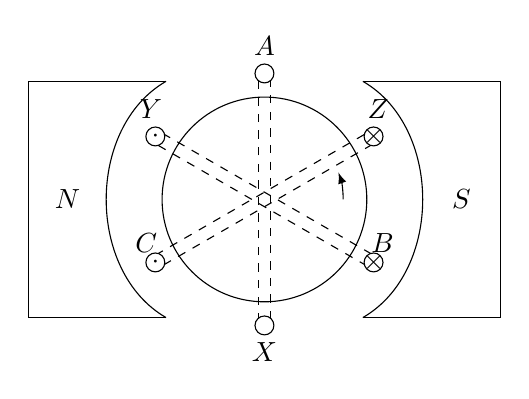
\begin{tikzpicture}[>=latex]
\draw (0,0) circle (1.3);

\foreach \x in {30,90,150}
{
    \draw [rotate=\x, dashed] (-1.6,-.08) rectangle (1.6,.08);
}
    \foreach \x in {30,90,150}
{        
    \draw (\x:1.6) [fill=white] circle (0.12);
    \draw (-\x:1.6) [fill=white] circle (0.12);
}

\node at (30:1.6){$\times$};
\node at (-30:1.6){$\times$};
\node at (150:1.6){$\cdot$};
\node at (-150:1.6){$\cdot$};

\draw [->] (1,0) arc (0:20:1);
\node at (32:1.7)[above]{$Z$};
\node at (-28:1.7)[above]{$B$};
\node at (150-2:1.7)[above]{$Y$};
\node at (-150-2:1.7)[above]{$C$};
\node at (90:1.7)[above]{$A$};
\node at (-90:1.7)[below]{$X$};

\draw (3,1.5)--(1.25,1.5);
\draw (3,-1.5)--(1.25,-1.5);
\draw (1.25,1.5) to [bend left=60](1.25,-1.5);
\draw (3,1.5)--(3,-1.5);
\draw (-3,1.5)--(-3,-1.5);
\draw (-3,1.5)--(-1.25,1.5);
\draw (-3,-1.5)--(-1.25,-1.5);
\draw (-1.25,1.5) to [bend left=-60](-1.25,-1.5);
\node at (-2.5,0){$N$};\node at (2.5,0){$S$};

\end{tikzpicture}
\caption{三相发电机的示意图}
\end{figure}

\begin{figure}[htp]\centering
\begin{circuitikz}[>=latex]
\draw (0,0)--(6,0) to [european, R=$1$] (6,2)--node[above]{$I_A$}(0,2)node[left]{$A$} to [american inductor] (0,0)node[left]{$X$};
\draw (-3+1,-2)node[left]{$C$} to [american inductor](0,-.25)node[left]{$Z$}--(6,-.25)--(6,-.5) to  [european, R=$3$] (3, -2)--(3,-3)--node[below]{$I_C$}(-3+1,-3)--(-3+1,-2);
\draw (.25,-.4)--(4.5*1.5-.5,-.4) to [european, R=2] (6.5*1.5-1, -2)--(6.5*1.5-1, -2.2)--node[below]{$I_B$}(1.5*1.5,-2.2)node[below]{$B$}to [american inductor] (.25,-.4)node[below]{$Y$};
\node at (-1+.5,-2-.5){发电机};\node at (6,-1.5){负载};
\end{circuitikz}
\caption{}
\end{figure}

图3.42是三相发电机的示意图.在铁心上固定着三个相同的线圈$AX$、$BY$、$CZ$,始端是$A$、$B$、$C$,末端是$X$、$Y$、$Z$.三个线圈的平面互成120$^\circ$角,匀速地转动铁心,三个线圈就在磁场里匀速转动,三个线圈是相同的,它们发出的三个电动
势,最大值和频率都相同,如果象图3.43那样把三个线圈分别跟负载连接起来,三相发电机就相当于三个独立的电源同时供电.

这三个电动势的最大值和频率虽然相同,但是它们的相位并不相同,由于三个线圈平面互成120$^\circ$角,所以三个电动势的相位也互差120$^\circ$.取图3.42所示的瞬间作为时间起点,这三个电动势可以分别表示为
\[\begin{split}
e_A&=\mathcal{E}_m\sin \omega t\\
e_B&=\mathcal{E}_m\sin (\omega t-120^\circ)\\
e_C&=\mathcal{E}_m\sin (\omega t-240^\circ)\\
\end{split}\]
它们的图象如图3.44所示.
\begin{figure}[htp]\centering
    \begin{tikzpicture}[>=latex, yscale=2]
\draw[<->] (0,1.5)node [right]{$e$}--(0,0)--(7,0)node[right]{$t$};
\draw [dashed](0,-1)--(2*3.1416,-1);
\draw [dashed](0,1)--(2*3.1416,1);
\foreach \x in {1,2,...,6}
{
    \draw [dashed](\x*3.1416/3, -1)--(\x*3.1416/3, 1);
}
\draw [ultra thick] plot[domain=0:2*3.1416, samples=1000] function{sin(x)} ;
\draw (0,0)--(0,-1.5);
\draw [ultra thick] plot[domain=0:2*3.1416, samples=1000] function{sin(x-3.1416*2/3)} ;
\draw [ultra thick] plot[domain=0:2*3.1416, samples=1000] function{sin(x+3.1416*2/3)} ;
\draw(3.1416*2/3,-1)--(3.1416*2/3,-1.5);
\draw [<->] (0,-1.3)--node[fill=white]{$\dfrac{T}{3}$}(3.1416*2/3,-1.3);
\node at (3.1416/2,1.2){$e_A$};
\node at (3.1416/2+3.1416*2/3,1.2){$e_B$};
\node at (3.1416/2+3.1416*4/3,1.2){$e_C$};




\end{tikzpicture}
\caption{}
\end{figure}

在实际应用中,三相发电机和负载都不是象图3.43那样连接,因为这种连接比起单相供电来没有什么优越之处,我们可以把图3.43中线圈末端和负载之间的三条导线合在一起,象图3.45那样用一条导线来连接,这样,每相负载上的电压不会改变,却可以节省两条导线.从每相线圈始端引出的导线叫做\textbf{端线},在照明电路里俗称火线,从公共点引出的导
线叫做\textbf{中性线},在照明电路里中性线是接地的,叫零线.这种有中性线的连接叫做\textbf{三相四线制}.照明电路通常采用三相四线制,灯泡连在端线和中性线之间(图3.46).
\begin{figure}[htp]\centering
\begin{circuitikz}
	\draw (0,0) to [american inductors, L] (0,2);
	\draw (0,0) to [american inductors, L] (-2,-1)node[left]{$C$};	
	\draw (0,0) to [american inductors, L] (2,-1)node[right]{$B$};	
	\draw[european] (5,0) to [R=1] (5,2);
	\draw [european](5,0) to [R=3] (-2+5,-1);	
	\draw[european] (5,0) to [R=2] (2+5,-1);				
	\draw(0,2)node[left]{$A$}--node [above]{端线}(5,2)	;
	\draw (2,-1)--(2,-1.5)--(2+5,-1.5)--(2+5,-1);		
	\draw (-2,-1)--(-2,-2)--(-2+5,-2)--(-2+5,-1);
	\draw (0,0)--node [above]{中性线}(5,0);
	\node at (0,.1) [left]{$O$};
	\node at (5,.1) [right]{$O'$};
	
	\node at (0,-1){发电机};
	\node at (5,-1.2){负载};
	\draw [fill=black](0,0) circle(1.5pt);	\draw [fill=black](5,0) circle(1.5pt);
\end{circuitikz}\caption{三相四线制}
\end{figure}

\begin{figure}[htp]\centering
    \begin{circuitikz}[>=latex,scale=1]
        \foreach \x in {1,2,3}
        {
            \draw [thick](-1.25,\x/2)--(-2,\x/2+.2);
            \draw (7,\x/2)--(1.5,\x/2) to [european, R] (0,\x/2) to [short, -o] (-1.25,\x/2);
            \draw  (-2,\x/2) to [short, o-o](-3,\x/2);
\draw [ultra thick](-3.25/2, 3/2+.1)--(-3.25/2, 1/2+.1);
        }
        \draw (7,0) to [short, -o](-3,0);
\node at (-3.5, 0){$O$}; \node at (-3.5, 0.5){$C$}; \node at (-3.5, 1){$B$}; \node at (-3.5, 1.5){$A$}; 
        \draw (.5, 0)to [short,*-](.5,-3); \draw (2.5, 0)to [short,*-](2.5,-3);\draw (4.5, 0)to [short,*-](4.5,-3);
        \draw (2, 1.5)to [short,*-](2,-3); \draw (4, 1)to [short,*-](4,-3);\draw (6, 0.5)to [short,*-](6,-3);

        \foreach \x in {-1,-2,-3}
        {
            \draw (.5,\x)to [lamp, *-*](2,\x);
            \draw (4.5,\x)to [lamp, *-*](6,\x);
            \draw (2.5,\x)to [lamp, *-*](4,\x);
        }
    \end{circuitikz}
\caption{三相四线制中灯泡的连接}
\end{figure}

\section{三相电路的连接}
现在我们进一步讨论三相电路的连接.先讨论电源的连接,然后讨论负载的连接.

\subsection{三相电源的连接}

在实际应用中,三相发电机的线圈通常都是采用图3.47所示的连接方法,这种连接方法叫做星形连接(符号是Y).这时电源提供两种电压,一种是每相线圈两端的电压,叫做\textbf{相电压};另一种是每两根端线之间的电压,叫做\textbf{线电压}(图3.47).在实际的发电机中,各相线圈的情况相同,所以三个相电压相等,通常用$U_{\text{相}}$来表示.这时三个线电压也相等,通常用$U_{\text{线}}$来表示.
\begin{figure}[htp]\centering
\begin{circuitikz}[>=latex]
	\draw (0,0) to [american inductors, L] (0,2);
	\draw (0,0) to [american inductors, L] (-1.5,-1)node[left]{$C$};	
	\draw (0,0) to [american inductors, L] (1.5,-1)node[below]{$B$};	
	
	\node at (0,.1) [left]{$O$};
	
	\draw (0,2)node[left]{$A$}--(5,2);\draw (0,0)--(5,0);
	\draw (1.5,-1)--(5,-1);\draw (-1.5,-1)--(-1.5,-1.5)--(5,-1.5);
	\draw[<->] (3,0)--node [fill=white]{$U_{\text{相}}$}(3,2);
		\draw[<->] (4,-1)--node [fill=white]{$U_{\text{线}}$}(4,2);
	\draw [fill=black](0,0) circle(1.5pt);
	\foreach \x in {0,2,-1,-1.5}
	{
		\draw[fill=white] (5,\x) circle({1.5pt});
	}
\end{circuitikz}\caption{电源的星形连接}
\end{figure}

在三相电源的星形连接中,相电压和线电压并不相等,这一点用伏特表测量一下就可以看出来,测量和计算表明,\textit{在
三相电源的星形连接中,线电压是相电压的$\sqrt{3}$倍},即
\[U_{\text{线}}=\sqrt{3}U_{\text{相}}\]

\subsection{负载的星形连接}


负载也可以采用星形连接,图3.45和图3.46中的负载就是星形连接的,在这种连接中,加在每相负载上的电压就是相电压(图3.48),通过每相负载的电流,可以利用交流电路中的欧姆定律计算出来,各相的负载不同,通过它们的电流也不相同,通过每相负载的电流叫做\textbf{相电流};通过端线的电流叫做\textbf{线电流}.在这种连接中,一根端线连接一相负载,各个线电流分别等于各个相电流.
\begin{figure}\centering
    \begin{circuitikz}[european,scale=.6,>=latex]
    
\draw (0,0) to [R=$2$, *-*] (2,-3) ;
\draw (0,0) to [R=$3$, *-*] (-2, -3);
\draw (0,0) to [R=$1$] (0,4);
\draw (0,4)--(-4-2,4);
\draw (-2,-3)--(-4-2,-3);
\draw (-4-2,-4)--(2,-4)--(2,-3);
\draw (0,0)--(-4-2,0);
\draw (0,4)--(-4-2,4);
\foreach \x in {0,-4,-3,4}
{
    \draw [fill=white] (-4-2,\x) circle (3pt);
}

\node at (-4.8-2,0){$O$};
\node at (-4.8-2,-4){$B$};
\node at (-4.8-2,-3){$C$};
\node at (-4.8-2,4){$A$};
\node at (.5,0){$O'$};
\draw [<->] (-3-2,0)--node[fill=white]{$U_{\text{相}}$}(-3-2,4);
\draw [->](-5,4)--(-4,4) node [above]{$I_{\text{线}}$};
\draw [->](0,4)--(0,3) node [right]{$I_{\text{相}}$};

    \end{circuitikz}
    \caption{负载的星形连接}
\end{figure}

中性线是三相负载的公共回线,通过的电流是三个相电流的总合,现在看一下三相负载相同时,通过中性线的电流.
例如三相负载是三个等值的电阻,或是三个相同的线圈,就属于负载相同的情况,图3.49表示在这种情况下三个相电流的曲线.三个电流的最大值和频率相同,位相互差120$^\circ$.从图中可以知道,三个相电流的总合在任何时刻都等于零,这一点,利用数学中学过的三角知识也可以得到证明,这就是说,在三相负载相同的情况下,在中性线里没有电流通过,既然
如此,中性线就可以省去不用了,这就成为\textbf{三相三线制}(图3.50).
\begin{figure}[htp]\centering
\begin{tikzpicture}[>=latex, yscale=1.6]
    %\draw [|<->|](3.7,1.4796)--node[fill=white]{$i_b$}(3.7,0);
%\draw [|<->|](3.3,-0.9534)--node[fill=white]{$i_c$}(3.3,0);
%\draw [|<->|](3.7,-.5262)--node[fill=white]{$i_a$}(3.7,0);

\draw[decorate,decoration=brace, thick](3.55,1.4796)--node[right]{$i_b$}(3.55,0);
\draw[decorate,decoration=brace, thick](3.55,0)--node[right]{$i_c$}(3.55,-0.9534);
\draw[decorate,decoration=brace, thick](3.45,-.5262)--node[left]{$i_a$}(3.45,0);


\draw[->] (0,-1.6)--(0,1.8)node [right]{$i$};
\draw [->](0,0)--(7,0)node [right]{$t$};
\draw [thick] plot [domain=0:3.1416*2, samples=1000] function{1.5*sin(x)} ;
\draw [very thick] plot [domain=0:3.1416*2, samples=1000] function{1.5*sin(3.1416*2/3+x)} ;
\draw [ultra thick] plot [domain=0:3.1416*2, samples=1000] function{1.5*sin(3.1416*4/3+x)} ;
\node at (3.1416/2, 1.7){$i_a$};
\node at (3.1416/2+3.1416*2/3, 1.7){$i_b$};
\node at (3.1416/2+3.1416*4/3, 1.7){$i_c$};



\draw[dashed](3.5, 1.4796)--(3.5,-0.9534);


\end{tikzpicture}
\caption{三相负载相同时的电流}
\end{figure}

\begin{figure}[htp]\centering
	\begin{circuitikz}
		\draw (0,0) to [american inductors, L] (0,2);
			\draw (0,0) to [american inductors, L] (-2,-1)node[left]{$C$};	
			\draw (0,0) to [american inductors, L] (2,-1)node[right]{$B$};	
		\draw[european] (5,0) to [R=1] (5,2);
\draw [european](5,0) to [R=3] (-2+5,-1);	
\draw[european] (5,0) to [R=2] (2+5,-1);				
\draw(0,2)node[left]{$A$}--(5,2)	;
	\draw (2,-1)--(2,-1.5)--(2+5,-1.5)--(2+5,-1);		
	\draw (-2,-1)--(-2,-2)--(-2+5,-2)--(-2+5,-1);
	
	\node at (0,.1) [right]{$O$};
	\node at (5,.1) [right]{$O'$};
	
	\node at (-1,-1.7){发电机};
	\node at (5,-1.2){负载};
			
	\end{circuitikz}\caption{三相三线制}
\end{figure}

三相三线制适用于负载相同的情况,下节要讲的感应电动机,它的三个定子线圈是相同的负载,这种电动机就可以接在三相三线制电路中(图3.51).在照明电路中,电灯的使用经常有变化,很难保证三相负载相同,必须用三相四线制.三相四线制比三相三线制多一根中性线,但可以提供两种电(220/380伏),照明和动力可以共用,相电压 220伏 供给照明,线电压380伏供给动力.
\begin{figure}[htp]\centering
\includegraphics[scale=.75]{fig/3-51.png}
\caption{电动机定子线圈的星形连接}
\end{figure}

\subsection{负载的三角形连接}

负载也可以如图3.52所示那样连接起来,这种连接方法叫做三角形连接(符号是$\triangle$),在这种连接中,加在每相负载上的电压是线电压,通过每相负载的相
电流也可以利用交流电路中的欧姆定律计算出来,各相负载相同时,三个相电流相等,通过端线的三个线电流也相等,显然,这时线电流不等于相电流,测量和计算表明,在负载的三角形连接中,三相负载相同时,线电流是相电流的$\sqrt{3}$倍,即
\[I_{\text{线}}=\sqrt{3}I_{\text{相}}\]
\begin{figure}\centering
    \begin{circuitikz}[european,scale=.8,>=latex]
    
\draw (0,0) to [R=$2$, *-*] (5,0) to [R=$1$, *-*] (2.5, 4) to [R=$3$] (0,0);
\draw (5,0)--(5,-2)--(-4,-2);
\draw (0,0)--(-4,0);
\draw (2.5,4)--(-4,4);
\foreach \x in {0,-2,4}
{
    \draw [fill=white] (-4,\x) circle (3pt);
}

\node at (-4.3,0){$C$};

\node at (-4.3,-2){$B$};
\node at (-4.3,4){$A$};
\draw [<->] (-3.5,0)--node[fill=white]{$U_{\text{线}}$}(-3.5,4);
\draw [->](-2,4)--(-1,4) node [above]{$I_{\text{线}}$};
\draw [->](2.5, 4)--(2,4-.8)node [left]{$I_{\text{相}}$};
\draw [->](2.5, 4)--(3,4-.8)node [right]{$I_{\text{相}}$};

    \end{circuitikz}
    \caption{负载的三角形连接}
\end{figure}

三相负载应该怎样连接,要看电源电压和负载额定电压的情况而定,例如对于线电压是380伏的三相电路,如果每相负载的额定电压是380伏,就用三角形连接;如果每相负载的额定电压是220伏,就用星形连接.

\subsection*{练习九}
\begin{enumerate}
    \item 根据图3.49写出三相负载相同时的相电流的瞬时值的表达式,并利用数学中学过的三角知识证明:三个相电流之和在任何时刻都等于零.
    \item 在图3.46所示的三相四线制电路中,相电压是220伏.现有“220V,100W”的灯泡90盏,第一相安装40盏,第二相安装30盏,第三相安装20盏.求灯泡全接通时,各个相电流和线电流.
    \item 如果电源采用图3.53所示的三角形连接,线电压和相电压的关系是怎样的?设各相线圈的情况相同.
\end{enumerate}
\begin{figure}[htp]\centering
\begin{circuitikz}
	\draw (0,0) to [american inductors, L] (-1.5, -2);
	\draw (0,0) to [american inductors, L] (1.5, -2);	
		\draw (1.5, -2) to [american inductors, L] (-1.5, -2);
	\draw (0,0)-- (4,0)node [right]{$A$};
	\draw (1.5, -2)-- (4,-2)node [right]{$B$};	
	\draw (-1.5, -2)--(-1.5, -3)-- (4,-3)node [right]{$C$};	
	\foreach \x in {-2,-3,0}
	{
		\draw[fill=white] (4,\x) circle({1.5pt});
	}
	\draw [fill=black](0,0) circle(1.5pt);
	\draw [fill=black](1.5, -2) circle(1.5pt);
	\draw [fill=black](-1.5, -2) circle(1.5pt);
\end{circuitikz}
\caption{}
\end{figure}


\section{感应电动机}
\subsection{旋转磁场}
\begin{figure}[htp]\centering
\includegraphics[scale=.75]{fig/3-54.png}
\caption{磁铁的旋转磁场}
\end{figure}

感应电动机是利用三相交流电可以产生旋转磁场以及电磁感应现象制成的.照图3.54那样,在磁铁中间放一个铝框,如果转动磁铁,造成一个旋转磁场,铝框就随着转动,磁铁转动时,铝框切割磁力线,其中产生感生电流,从楞次定律知道,感生电流和磁铁磁场的相互作用,要阻碍磁铁
和铝框的相对运动,现在磁铁是在外力作用下转动的,结果不是铝框阻止磁铁的转动,而是铝框被磁铁带着转动起来.
\begin{figure}[htp]\centering
\includegraphics[scale=.75]{fig/3-55.png}
\caption{三相电的旋转磁场}
\end{figure}

不仅转动磁铁可以产生旋转磁场,三相交流电也可以产生旋转磁场.取三个相同的线圈,照图3.55那样使它们的平面交成120$^\circ$角,线圈中通以三相交流电,中间的铝框就象被转动的磁铁带着一样转动起来,说明三相交流电也产生旋转磁场.
\begin{figure}[htp]\centering
\begin{tikzpicture}[>=latex, scale=1.6]
    \draw[->] (0,-1.3)--(0,1.5)node [right]{$i$};
    \draw [->](0,0)node[left]{$O$}--(7,0)node [right]{$t$};
    \draw [very thick] plot [domain=0:3.1416*2, samples=1000] function{0.9*sin(x)} ;
    \draw [very thick] plot [domain=0:3.1416*2, samples=1000] function{0.9*sin(3.1416*2/3+x)} ;
    \draw [very thick] plot [domain=0:3.1416*2, samples=1000] function{0.9*sin(3.1416*4/3+x)} ;
    \node at (3.1416/2, 1.2){$i_{AX}$};
    \node at (3.1416/2+3.1416*2/3, 1.2){$i_{BY}$};
    \node at (3.1416/2+3.1416*4/3, 1.2){$i_{CZ}$};
\draw[dashed] (3.1416*2/3, -1)--(3.1416*2/3, 1);
\draw[dashed] (3.1416*4/3, -1)--(3.1416*4/3, 1);
\draw[dashed] (3.1416*6/3, -1)--(3.1416*6/3, 1);
\node at  (3.1416*2/3+.2, 0)[below]{$\frac{1}{3}T$};
\node at  (3.1416*4/3+.2, 0)[below]{$\frac{2}{3}T$};
\node at (3.1416*6/3+.2, 0)[below]{$T$};
    \end{tikzpicture}
\includegraphics[scale=.75]{fig/3-56.png}
\caption{旋转磁场的产生}
\end{figure}

现在用图3.56来说明三相交流电为什么会产生旋转磁场.在开始的时刻($t=0$),即在图3.56甲所示的瞬间,线圈$AX$中的电流$i_{AX}$是零;线圈$BY$中的电流$i_{BY}$是负值,电流从末端$Y$流向始端$B$;线圈$CZ$中的电流$i_{CZ}$是正值,电流从始端$C$流向末端$Z$.电流$i_{BY}$、$i_{CZ}$形成的合成磁场如图中的虚线所示,方向指向$A$.

经过$T/3$,在图3.56乙所示的瞬间,线圈$AX$中的电流
$i_{AX}$是正值,电流从始端$A$流向末端$X$;线圈$BY$中的电流$i_{BY}$是零;线圈$CZ$中的电流$i_{CZ}$是负值,电流从末端$Z$流向
始端$C$.电流$i_{AX}$、$i_{CZ}$形成的合成磁场如图中的虚线所示,方向指向$B$.可以看出,磁场方向沿逆时针转过120$^\circ$角.

图3.56丙和丁分别表示经过$2T/3$和$T$时,各个线圈中电流的方向和合成磁场的方向.可以看出,每经过$T/3$,磁场方向就沿逆时针转过120$^\circ$角.在交流电的一周期内磁场旋转一周.

\subsection{感应电动机}

感应电动机是利用图3.55中的现象制成
的,它有一个定子(图3.57甲)和一个转子(图3.57乙),在定子内侧的凹槽里联有互成120$^\circ$角的三组线圈(定子绕组),把这三组线圈用星形接法或三角形接法连入三相电路中,就产生旋转磁场.
\begin{figure}[htp]\centering
\includegraphics[scale=.75]{fig/3-57.png}
\caption{感应电动机的定子和转子}
\end{figure}

感应电动机的转子是由铁心和嵌在铁心上的闭合导体构成的,闭合导体是由嵌在铁心凹槽中的铜条(或铝条)和两个铜环(或铝环)连在一起制成的,形状象个鼠笼(图3.57丙),
所以这种电动机也叫鼠笼式感应电动机,这个闭合导体相当于图3.56中的铝框,有了旋转磁场,它就转动起来.

鼠笼式感应电动机的构造简单,要改变转动方向,只要把定子上的任意两组线圈的电流互换一下就行了.这种电动机制造、使用、保养都比较简单,广泛应用在工农业生产中.能够使用鼠笼式感应电动机,是三相交流电的另一个优点.

\section*{阅读材料:直线电机和磁悬浮列车}

一般电动机工作时都是转动的,但是用旋转电机来驱动
的交通工具要做直线运动,用旋转电机来驱动的机器的一些部件也要做直线运动.这就需要有把旋转运动变为直线运动的一套装置.能不能直接利用直线运动来驱动,而省去这套装置呢?几十年前人们就提出了这个问题,现在已制成了利用直线运动的电动机,即直线电机.

直线电机的原理并不复杂.设想把一台旋转感应电动机沿着一条半径的方向剖开,并且展平,就成了一台直线感应电动机(图3.58),在直线电机中,相当于旋转电机定子的,叫初级;相当于旋转电机转子的,叫次级.初级中通以交流电,
次级在电磁力的作用下就沿着初级做直线运动,这时初级要做得很长,延伸到运动所需要达到的位置,而次级不需要那么长,实际上,直线电机既可以把初级做得很长,也可以把次级做得很长;既可以初级固定、次级移动,也可以次级固定,初级移动.
\begin{figure}[htp]\centering
\includegraphics[scale=.75]{fig/3-58.png}
\caption{由旋转电机到直线电机}
\end{figure}

直线电机是一种新型电机,近年来应用日益广泛,磁悬浮列车就是用直线电机来驱动的.磁悬浮列车是一种新型列车,是铁路技术中一项新兴的技术成果,一般的列车由于车轮和铁轨之间有摩擦,所能达到的最高运行速度为300$\kmh$左右,要超过这个速度,用旋转电机来驱动并不理想,用直线电机来驱动却很含适,直线电机的一个级固定于地面,跟导轨一起延伸到远处;另一个级安装在列车上,初级通以交流电,列车就沿导轨前送.同时利用磁悬浮使列车跟导轨脱离接触,减小摩擦.列车上装有磁体(有的就是兼用直线电机的线圈),磁体随列车运动时,使设在地面上的金属板或线圈中出现感生电流,利用磁体和感生电流之间的电磁力把列车悬浮起来,有的国家已建立了几千米的磁悬浮列车试验线,运行速度高达500$\kmh$以上.人们预计,本世纪末磁悬浮列车可达到实用化的阶段.

直线电机除了用于磁悬浮列车,还可广泛地用于其他方
面,如用于传送系统、电气锤、电磁搅拌器等.在我国,直线电视也逐步得到推广和应用.直线电机的原理虽然不复杂,但在设计、制造方面有它自己的特点,产品还不如旋转电机那样成熟,有待进一步研究和改进.

\subsection*{练习十}
\begin{enumerate}
    \item 有一台感应电动机,铭牌上标有“220/380”“$\triangle$/Y”的字祥.这表示这台电动机每相定于线圈的额定电压是 220伏,如果线电压是220伏,定子线圈要连成三角形;如果线电压是380伏,定子线圈要连成星形,为什么?
    \item 实验表明:只要把定子上任意两组线圈的电流互换一下,旋转磁场就向相反方向旋转.画出类似于图3.56的
    图,并加以分析说明.
    \item 在图3.54所示的实验中,铝框总要比磁铁转得慢,即比旋转磁场转得慢,而不能跟磁场转得一样快,即不能同步旋转,因此感应电动机也叫异步电动机,试说明铝框为什么不能跟磁铁同步旋转.
\end{enumerate}

\section*{复习题}
\begin{enumerate}
\item 就图3.1所示的装置简述正弦交流电的产生和正弦交流电的变化规律,
\item 表征正弦交流电的三个物理量是什么?什么叫交流电的最大值和有效值?对正弦交流电来说,二者之间有什么关系?什么叫做交流电的相和初相?什么叫做相差?
\item 纯电阻电路中欧姆定律的表达式是怎样的?功率的表达式是怎样的?电阻对交流电的电流和电压的相位关系有没有影响?
\item 纯电感电路中欧姆定律的表达式是怎样的?感抗跟
自感系数和交流电频率间有什么关系?电感线圈在电路中表现出什么特性?
\item 纯电容电路中欧姆定律的表达式是怎样的?容抗跟电容和交流电频率间有什么关系?电容器在电路中表现出什么特性?
\item 纯电感电路中,电流和电压的相位关系是怎样的?在纯电容电路中,电流和电压的相位关系是怎样的?
\item 交流电的功率表达式是怎样的?什么叫有功功率、视在功率和功率因数?
\item 简述变压器的工作原理.变压器原副线圈上的端电压之比等于什么?原副线圈中的电流之比等于什么?
\item 简述电能输送的原理.
\item 简述交流电整流和滤波的原理和方法.
\item 简述三相交流电的产生,在电源的星形连接中,线电压和相电压的关系是怎样的?在负载的星形连接中,线电流和相电流的关系是怎样的?在负载的三角形连接中,线电流和相电流的关系是怎样的?
\item 简述感应电动机的原理.
\item 你自己总结一下,交流电比直流电有哪些优点.
\item 你自己总结一下,交流电和直流电存在什么共同点,交流电又有什么特点,哪些规律形式相同,哪些规律有所不同.
\end{enumerate}

\section*{习题}
\begin{enumerate}
    \item 把电阻和电容器串联在交流电路中,测得电阻上的电压为30伏,电容器上的电压为40伏.已知电阻的阻值为200欧,交流电的频率为50赫,求电容器的电容,这道题提供了一种用伏特表测定电容的方法.
    \item 把电阻和电容器并联在交流电路中,已知电阻的阻值是500欧,电容器的电容是30微法.当交流电的频率为50赫时,通过电阻和电容器的电流之比是多大?当交流电的频率是500赫时,电流之比又是多大?
    \item 变压器的原线圈为1100匝,副线圈为180匝,原线圈接到220伏的交流电路中,副线圈上并联了3个阻值都是90欧的用电器.如果原线圈允许通过的最大电流为0.9安,副线圈上最多还可以并联多少个阻值为60欧的用电器?
    \item 有一个教学用的可拆变压器,它的原副线圈外部还可绕线,现在要测定原副线圈的匝数.现有一根足够长的绝缘导线,还需要什么器材?简要说明实验原理.
    \item 图3.59是电工常用的钳形电流表,可以用来测定交变电流,把钳口打开,把被测的通电导线放在钳口中间(右图),交流电表就可以测出导线中的电流强度.试说明钳形电流表的工作原理.
\begin{figure}[htp]\centering
\includegraphics[scale=.75]{fig/3-59.png}
\caption{钳形电流表}
\end{figure}
    \item 在图3.35所示的桥式整流电路中,变压器原副线圈的匝数比等于8,原线圈接在220伏的交流电路中,能不能选用最高反向工作电压为50伏的晶体二极管进行整流?为什么?
    \item 图3.60是电子技术中用到的限幅电路,电池组的电动势都为$\mathcal{E}$,左端输入的是正弦交流电,电压$u_1$的最大值为$2\mathcal{E}$.试画出右端输出的电压$u_2$的图象,并分析说明理由.电池组的内电阻略去不计.
\begin{figure}[htp]\centering
\begin{circuitikz}[>=latex, european, scale=.8]
\draw (0,0)--(3,0)--(5,0)--(7,0);
\draw (0,4)to [R=$R$](3,4)--(5,4)--(7,4);
\ctikzset{diodes/scale=0.6}\draw (3,4) to [full diode ] (3,2) to [battery] (3,0);
\ctikzset{diodes/scale=0.6}\draw (5,0) to  [battery] (5,2) to [full diode ](5,4);

\node at (2.3,3){$D_1$};\node at (5.7,3){$D_2$};

\draw [fill=white] (0,0) circle (2.5pt);
\draw [fill=white] (0,4) circle (2.5pt);
\draw [fill=white] (7,0) circle (2.5pt);
\draw [fill=white] (7,4) circle (2.5pt);
\draw [fill=black] (3,0) circle (2.5pt);
\draw [fill=black] (3,4) circle (2.5pt);
\draw [fill=black] (5,0) circle (2.5pt);
\draw [fill=black] (5,4) circle (2.5pt);

\draw[<->](0,.1) to node [fill=white]{$u_1$} (0,3.9);
\draw[<->](7,.1) to node [fill=white]{$u_2$} (7,3.9);
\end{circuitikz}
\caption{二极管限幅电路}
\end{figure}
    \item 在图3.46所示的三相四线制照明电路中,设$A$相接通了8盏“220V,100W”的灯泡,$B$相接通了2盏“220V,100W”的灯泡,$C$相中没有接通灯泡,这时接通的灯泡都正常发光,因某种原因中性线断开了(在该图中$O$处断开),将会发生什么现象?说明理由.
    
    在三相四线制电路中,中性线在任何时候都不能断开.
    为了避免中性线断开,在中性线上也不能安装开关和保险丝.做完这道题,你将会对此有所了解.
    \item 如图3.61所示,电源采用星形连接,负载采用三角形连接.电源的相电压是220伏,各相负载相同,阻值都是110欧,求通过各相负载的相电流和线电流.
\begin{figure}[htp]\centering
	\begin{circuitikz}
	\draw (0,0) to [american inductors, L] (0,2);
	\draw (0,0) to [american inductors, L] (-2,-1)node[left]{$B$};	
	\draw (0,0) to [american inductors, L] (2,-1)node[right]{$C$};	
	\draw[european] (5,2) to [R] (3,-1);
	\draw [european](5,2) to [R] (7,-1);	
	\draw[european] (3,-1) to [R] (7,-1);				
	\draw(0,2)node[left]{$A$}--(5,2)	;
	\draw (2,-1)--(2,-1.5)--(2+5,-1.5)--(2+5,-1);		
	\draw (-2,-1)--(-2,-2)--(-2+5,-2)--(-2+5,-1);
	
\end{circuitikz}\caption{}
\end{figure}
    \item 每一台电动机都有一定的额定功率.在实际中要根据负载的功率来选择电动机的功率,使电动机的额定功率等于或稍大于负载的功率,有一台水泵,抽水量$Q=0.03{\rm m^3}/{\rm s}$,抽水高度$h=20{\rm m}$,效率$\eta_1=0.55$,用一台感应电动机道过皮带传动来带动,皮带传动的效率$\eta_2=0.8$.现有三台感应电动机,额定功率分别是14千瓦、20千瓦、28千瓦,应当选择哪一台?计算时取$g=10\msq$.
\end{enumerate}

































